\documentclass[11pt,a4paper]{article}
\usepackage[a4paper,margin=2.2cm]{geometry}
\usepackage[T1]{fontenc}
\usepackage{lmodern}
\usepackage{microtype}
\usepackage{amsmath,amssymb}
\usepackage{graphicx}
\usepackage{booktabs}
\usepackage{tabularx}
\usepackage{multirow}
\usepackage[table]{xcolor}
\usepackage{caption}
\usepackage{subcaption}
\usepackage{tikz}
\usetikzlibrary{arrows.meta,positioning}
\usepackage{enumitem}
\usepackage[section]{placeins}
\usepackage[hidelinks]{hyperref}
\usepackage{url}
\def\UrlBreaks{\do\/\do-\do\_}

\captionsetup{font=small,labelfont=bf}
\setlist{nosep,leftmargin=1.4em}
\newcolumntype{Y}{>{\raggedright\arraybackslash}X}
\newcommand{\ci}[2]{{\footnotesize[#1,\,#2]}}
\newcommand{\sg}{\operatorname{sg}}
\renewcommand{\arraystretch}{1.12}
\newcommand{\repo}{https://github.com/dhyan2004-dot/Exploring-Adversary-Strategies-in-Object-Detection}

\title{\textbf{A Comparative Study of Robustness- and Naturalness-Aware Adversarial Patch Attacks for UAS Object Detection}}
\author{Dhyan G \quad (AE22B030)\\[2pt]\small AE5510 Security of Safety-Critical Systems --- Final Project Report}
\date{20 November 2026}

\makeatletter\setlength\@fptop{0pt}\setlength\@fpsep{14pt plus 2pt}\setlength\@fpbot{0pt plus 1fil}\makeatother
\begin{document}
\maketitle

\begin{abstract}
This project designs physical-domain adversarial attacks against an object detector deployed on an uncrewed aircraft system (UAS), using a dataset of aerial images with four classes (Aircraft, Military Truck, Tank, Building). A YOLOv8s detector is fine-tuned as the baseline, and an object-disappearance attack with a printable adversarial patch is developed for the Tank class. Three patch-generation strategies are compared on the same detector, data and evaluation: a standard Expectation-over-Transformation (EOT) patch, the Pattern Corruption-Assisted attack (CPA), which adds light-spot and shadow corruptions during optimisation to improve robustness and transferability, and the Naturalistic Physical Adversarial patch (NPA), which restricts the patch to the output of a pretrained GAN to make it look natural. CPA is re-implemented as a 3-D roof texture with a 1\,m printable sheet that always lies on the vehicle, and every attack is tested on three black-box detectors (YOLOv8m, YOLO11s, RT-DETR-l). Because the 3,168 training images are augmentations of only 88 source photographs, all results use 5-fold cross-validation grouped by photograph, same-size gray and noise sheets as occlusion controls, and photo-level confidence intervals. The attack removes almost all Tank detections from the full-image metric (Tank AP50 $0.156\to0.009$, against $0.052$ for a gray square) while leaving the other classes unchanged; the 1\,m 3-D sheet hides 12--27 percentage points more tanks than a gray sheet on all four detectors, and about half of the effect transfers to unseen detectors. The added structure of CPA gives no measurable benefit: corruption training changes black-box success by $-0.004$ \ci{$-0.02$}{$+0.01$}, also under four ablations. NPA's latent constraint alone does not keep patches natural; with a naturalness-budget early stop it yields photo-like patches that keep half the attack and 70\,\% of it on unseen detectors.
\end{abstract}

\noindent{\small\textbf{Code repository:} \url{\repo}}

%=====================================================================
\section{Introduction}\label{sec:intro}

\subsection{Problem}
The task is to design physical-domain adversarial attacks against the object detector of a UAS, using the course dataset of aerial images with four categories: Aircraft, Military Truck, Tank and Building. The project has four required parts: (i) select and fine-tune a state-of-the-art detector and establish its clean baseline with precision, recall, AP and mAP on the validation and test data; (ii) generate a physically realisable perturbation that causes misclassification or disappearance of a target object, using the training set and constraints that make it robust to viewing angle, scale, illumination and distance; (iii) evaluate the effectiveness and transferability of the perturbation on held-out data with the same metrics; and (iv) quantify the degradation of detection performance relative to the baseline across the object categories.

\subsection{Motivation and approach}
An attacker who wants to hide a vehicle from an airborne detector can only change the physical scene, for example by placing a printed sheet on the vehicle; the image is then formed by a camera at an unknown altitude, angle and illumination. A perturbation optimised for one image does not survive these changes, so the attack has to be optimised in expectation over them (EOT \cite{athalye2018}), which is the standard baseline. Two published methods claim to improve on it in exactly the directions the project asks about. CPA \cite{zhang2024cpa}, proposed for UAV remote sensing, adds light spots and shadows during optimisation and reports better robustness and \emph{transferability} to detectors the attacker cannot access. NPA \cite{hu2021npa} generates the patch with a pretrained GAN so that it looks like a natural image, which matters for a physical attack because an obviously adversarial pattern can be noticed by a human analyst. The project therefore compares the three strategies under one detector, dataset and evaluation, and asks whether the additional structure of CPA or NPA gives a measurable benefit over a standard EOT patch.

Two properties of the data shaped the method. First, only images and boxes are available, so the physical attack is simulated digitally: the patch is rendered into real aerial photographs under sampled viewpoints, scales and corruptions, rather than printed and flown. Second, the training set contains 3,168 files but only 88 distinct source photographs; without care, augmented copies of a test photograph end up in training and every metric is inflated. The evaluation is designed around both facts (Section~\ref{sec:eval}).

\subsection{Questions addressed}
\begin{enumerate}
  \item How much does an adversarial patch degrade the detector, per class and beyond what plain occlusion achieves?
  \item Does corruption-assisted optimisation (CPA) improve robustness under simulated physical variations and transfer to other detectors?
  \item Can latent-space optimisation (NPA) give natural-looking patches without losing the attack?
  \item Do patches optimised on YOLOv8 transfer to other architectures (the case where the defender's model is unknown)?
  \item Which conditions (lighting, shadow, rain, mud, patch size) change the attack, and how?
\end{enumerate}

%=====================================================================
\section{Literature review}\label{sec:lit}

\paragraph{Adversarial and physical attacks.} Small, structured input changes can change the output of neural networks \cite{szegedy2014,goodfellow2015}, and such changes survive printing and re-photographing \cite{kurakin2017}. Physical attacks restrict the change to an object that can be manufactured: eyeglass frames with a total-variation smoothness term and a printability constraint \cite{sharif2016}, stickers on road signs \cite{eykholt2018}, and the universal adversarial patch \cite{brown2017}. Athalye et al.\ \cite{athalye2018} introduced EOT, optimising the expected loss over a distribution of physical transformations (Eq.~\ref{eq:eot}).

\paragraph{Attacks on object detectors.} A detector predicts thousands of candidate boxes with class scores and then removes duplicates with non-maximum suppression (NMS); because NMS and thresholding are not differentiable, attacks minimise the raw candidate scores. ShapeShifter \cite{chen2018shapeshifter} attacked Faster R-CNN with printed signs, and Thys et al.\ \cite{thys2019} hid people from YOLOv2 with a printed patch, the template for most later patch attacks; wearable attacks added cloth deformation \cite{xu2020tshirt,wu2020cloak}. For vehicles, textures are optimised on 3-D models through a differentiable renderer, which maps a texture to image pixels for a given camera and propagates gradients back to the texture: UPC \cite{huang2020upc}, DAS \cite{wang2021das}, FCA \cite{wang2022fca} and DTA \cite{suryanto2022dta}.

\paragraph{Aerial detectors.} Den Hollander et al.\ \cite{denhollander2020} hid aircraft in overhead imagery with patches, and Du et al.\ \cite{du2022aerial} attacked an aerial car detector with physical patches and real UAV flights, reporting that lighting strongly affects success. Tang et al.\ \cite{tang2024de} attacked aerial detectors in a black-box setting with differential evolution. CPA \cite{zhang2024cpa} renders a texture on an auxiliary mesh on a simulated car (CARLA) and adds \emph{pattern corruptions} (a light spot on the target, a shadow around it, each with probability 0.5) to the training images. The authors argue that the corruptions push training images towards the detector's decision boundary, which different detectors share, so the patch transfers better; their ablation reports 15.5\,\% $\to$ 20.8\,\% transfer success with light and shadow. Rain and mud are used only as unseen test corruptions, following common-corruption benchmarks \cite{hendrycks2019}.

\paragraph{Transferability.} Adversarial examples made on one model often fool another \cite{liu2017transfer}; random input transformations during optimisation improve this by preventing overfitting to the surrogate model \cite{xie2019di}. CPA's corruptions are such a transformation, which is the hypothesis examined in Section~\ref{sec:res-why}.

\paragraph{Natural-looking patches.} PS-GAN \cite{liu2019psgan} generated patches with a GAN conditioned on a seed image. NPA \cite{hu2021npa} optimises only the latent input of a pretrained BigGAN \cite{brock2019} and bounds every latent component by $\tau$ to control realism. AdvCaT \cite{hu2023advcat} restricts the texture to a few camouflage colours in irregular regions, so the result is natural by construction; diffusion-model patches \cite{lin2023diffusion} are a recent alternative.

\paragraph{Evaluation methodology.} Placing augmented copies of one image on both sides of a split is data leakage \cite{kaufman2012}; grouped cross-validation is the remedy for clustered data \cite{roberts2017}, uncertainty must then be estimated at the cluster level \cite{field2007}, and training randomness alone can change benchmark results, so repeated runs are needed \cite{bouthillier2021}.

\paragraph{Gap.} The UAV attacks above were evaluated in simulation or on few physical scenes, without occlusion controls and with one training run per configuration. Whether corruption training improves transfer, and whether a GAN prior keeps an aerial patch natural, has not been tested on real aerial photographs with such controls.

%=====================================================================
\section{Methodology}\label{sec:method}

\subsection{Detection metrics}\label{sec:metrics}
A prediction is a true positive if its class is correct and its intersection-over-union with an unmatched ground-truth box is at least a threshold $t$, $\mathrm{IoU}(A,B)=|A\cap B|/|A\cup B|$. Sorting predictions by confidence gives precision $P=\mathrm{TP}/(\mathrm{TP}+\mathrm{FP})$ and recall $R=\mathrm{TP}/(\mathrm{TP}+\mathrm{FN})$ as functions of the confidence cut-off. The average precision of a class is the area under the precision envelope,
\begin{equation}
\mathrm{AP}_t=\int_0^1\tilde p(r)\,dr,\qquad \tilde p(r)=\max_{r'\ge r}p(r'),
\end{equation}
mAP50 is the mean of $\mathrm{AP}_{0.5}$ over classes, and mAP50-95 also averages over $t=0.50,0.55,\dots,0.95$, rewarding tight boxes. Reported precision and recall are at the confidence that maximises F1, as computed by Ultralytics.

\subsection{Threat model and attack objective}
The attack is an \emph{object-disappearance} attack on class Tank: one universal patch $P$ is placed on each tank so that the detector no longer reports a tank there. Disappearance is chosen over targeted misclassification because, for airborne surveillance, an unreported vehicle is the failure that propagates silently; a tank relabelled as another class also counts as hidden, so misclassification is included. In the \emph{white-box} setting the attacker can back-propagate through the detector (the surrogate, YOLOv8s); in the \emph{black-box} setting the patch is evaluated on detectors that were not used to create it (YOLOv8m, YOLO11s, RT-DETR-l). With $\mathcal{D}$ the tanks the detector reports before patching (confidence $\ge c$, IoU $\ge0.3$ with the label), the attack success rate is
\begin{equation}
\mathrm{ASR}=\frac{1}{|\mathcal{D}|}\sum_{i\in\mathcal{D}}\mathbb{1}\big[\,\mathrm{conf}_i(\text{patched})<c\,\big],
\end{equation}
with $c=0.5$ as in CPA (0.25 for the 2-D stage). Tank is the target because it is the class the detector finds reliably (Section~\ref{sec:res-det}); Military Truck is almost never detected (AP50 $\approx0.07$), so there is nothing to hide, and a sheet on a building has no comparable physical meaning. Aircraft is attacked as a second class in the 2-D stage.

\subsection{Data}\label{sec:data}
Labels contain both YOLO boxes and 4-point polygons; polygons are converted to their axis-aligned bounding boxes and degenerate boxes removed. All augmented copies of a source photograph share a 32-character hash in their file name, which identifies the 88 source photographs. The official Validation and Testing splits contain 16 images each and share no photograph with the training pool.

\subsection{Evaluation design}\label{sec:eval}
\paragraph{Photo-grouped cross-validation.} A first validation split made file by file gave mAP50 $=0.86$ while the official test split gave 0.20, because augmented siblings of the validation photographs were in training. All experiments therefore use 5-fold cross-validation over photographs: each photograph $g$ is assigned to one fold $k(g)$ (rare classes first, balanced per class), and in round $k$ every model (detector and patch) is trained on photographs with $k(g)\neq k$ and evaluated on fold $k$. Each photograph is tested exactly once by models that never saw it, so results are pooled over folds. The held-out folds serve as the validation data; the official test split is kept as an independent check.

\paragraph{Occlusion controls.} Any sheet that covers part of a vehicle can hide it. Every patch is evaluated next to a uniform gray sheet and a uniform-noise sheet of the same size, placement, rendering and corruption draw, and the reported effect is the
\begin{equation}
\text{margin}=\mathrm{ASR}_{\text{patch}}-\max\big(\mathrm{ASR}_{\text{gray}},\mathrm{ASR}_{\text{noise}}\big),
\end{equation}
the part attributable to the adversarial pattern rather than to covering the vehicle.

\paragraph{Photo-level statistics.} Tanks of one photograph share scene, lighting and viewpoint and are not independent. For photographs $g=1..G$ with $n_g$ evaluated tanks and $h_g$ hidden ones, a \emph{cluster bootstrap} \cite{efron1993,field2007} draws $G$ photographs with replacement, $\mathcal{S}^{*}_b$, and recomputes
\begin{equation}
r^{*}_b=\sum_{g\in\mathcal{S}^{*}_b}h_g\Big/\sum_{g\in\mathcal{S}^{*}_b}n_g,\qquad b=1..4000,
\end{equation}
and the 2.5 and 97.5 percentiles of $r^*_b$ (or of the margin) give the 95\,\% interval. Two methods $A,B$ on the same tanks are compared by a \emph{paired sign-flip test} \cite{good2005} on per-photo differences $d_g=\sum_{i\in g}(h^B_i-h^A_i)$: under no difference each $d_g$ is equally likely to be positive or negative, so
\begin{equation}
p=\frac{1}{2^{G'}}\sum_{s\in\{\pm1\}^{G'}}\mathbb{1}\Big[\big|\textstyle\sum_g s_gd_g\big|\ge\big|\sum_g d_g\big|\Big],
\end{equation}
over the $G'$ photographs with $d_g\ne0$ (exact up to $G'=16$, otherwise 20,000 random sign vectors). When $m$ tests are made together, Holm's correction \cite{holm1979} controls the probability of any false positive: with sorted $p_{(1)}\le\dots\le p_{(m)}$, $\tilde p_{(i)}=\max_{j\le i}\min\{1,(m-j+1)p_{(j)}\}$.

\subsection{Detectors}\label{sec:detectors}
YOLOv8s \cite{yolov8} was chosen as the surrogate: it is a current one-stage detector with a differentiable PyTorch implementation, fast enough for the many forward--backward passes of patch optimisation. It is initialised from COCO \cite{coco} and fine-tuned per fold at 960\,px with the first 10 layers (the backbone) frozen, batch 16, at most 15 epochs and early stopping (patience 5). Freezing and early stopping limit memorisation of the roughly 70 training photographs per fold; 960\,px gives small tanks more pixels than the default 640\,px. A 1280\,px variant and a backbone initialised from DOTA aerial weights \cite{xia2018dota} were also tested. The black-box detectors are a larger CNN of the same family (YOLOv8m), a newer CNN (YOLO11s) and a transformer detector (RT-DETR-l \cite{zhao2024rtdetr}, which predicts a fixed set of boxes with attention instead of dense anchors), each fine-tuned on the same folds; the architectural spread tests transfer from easy (same family) to hard (different paradigm).

\subsection{Stage 1: two-dimensional EOT and CPA patches}\label{sec:2d}
A $128\times128$ RGB patch is optimised on crops around each tank (2.5$\times$ the box, resized to $320\times320$). Crops are used because in convoy scenes a full-image loss is dominated by the other, unpatched tanks. Following Eq.~\eqref{eq:eot},
\begin{equation}
\min_{P\in[0,1]^{3\times128\times128}}\;\mathbb{E}_{t\sim\mathcal{T}}\Big[\frac{1}{|\mathcal{K}|}\sum_{i\in\mathcal{K}}\max_a s_a\big(A(x_i,P,t)\big)\Big]+\lambda\,\mathrm{TV}(P),\qquad\lambda=0.005,\label{eq:eot}
\end{equation}
where $s_a$ is the raw (pre-NMS) Tank score of candidate $a$, $\mathcal{K}$ the crops whose clean peak score is at least 0.25 (a tank the detector does not see gives no useful gradient), and $\mathcal{T}$ samples rotation $\pm20^\circ$, side $0.4w(1\pm0.2)$, brightness $\pm0.15$, contrast $0.85$--$1.15$ and position $\pm10\,\%$. The maximum is used because NMS keeps the highest-scoring candidate, so this is the detection that would survive. Total variation,
\begin{equation}
\mathrm{TV}(P)=\overline{|P_{:,i+1,j}-P_{:,i,j}|}+\overline{|P_{:,i,j+1}-P_{:,i,j}|},
\end{equation}
suppresses pixel-level noise that a printer and a distant camera would blur away \cite{sharif2016}. The CPA variant of this stage corrupts the patch during training (light, shadow, or both, probability 0.8) as a differentiable blend $P\leftarrow P(1-\alpha M)+\alpha Mc$ with mask $M\in[0,1]$, colour $c$ and strength $\alpha$. The masks are: \emph{light}, a Gaussian blob $M=\exp(-\|u-u_0\|^2/2\sigma^2)$ at a random centre ($\sigma=0.15$--$0.4$ of the side) towards warm white, $\alpha=0.4$--$0.9$; \emph{shadow}, a soft half-plane $M=1/(1+e^{-d/s})$, with $d$ the signed distance to a random line and edge softness $s$, towards black, $\alpha=0.3$--$0.7$; \emph{rain}, 25--80 thin tilted pale streaks; \emph{mud}, thresholded smooth noise covering 20--45\,\% of the patch in brown. Masks are drawn with NumPy and only the blend touches $P$, so gradients reach every pixel. Rain and mud are used only for testing, and the \emph{mixed} test condition stacks two random corruptions. Optimisation uses Adam (learning rate 0.01, 80 epochs of 600 tanks, three seeds). This stage showed that a pattern beats occlusion (Section~\ref{sec:res-2d}) but has three limitations: the patch (0.4 of the box width, up to $\approx2.8$\,m on a tank seen side-on) is too large to print, it can extend beyond the vehicle, and corrupting the patch is not the CPA method, which corrupts the scene around a 3-D texture. Stage 2 removes all three.

\subsection{Stage 2: three-dimensional CPA}\label{sec:cpa3d}
Figure~\ref{fig:pipeline} shows one training step. The components follow the authors' code; the changes needed for real photographs are the viewpoint sampling and the placement.

\begin{figure}[htbp]
\centering
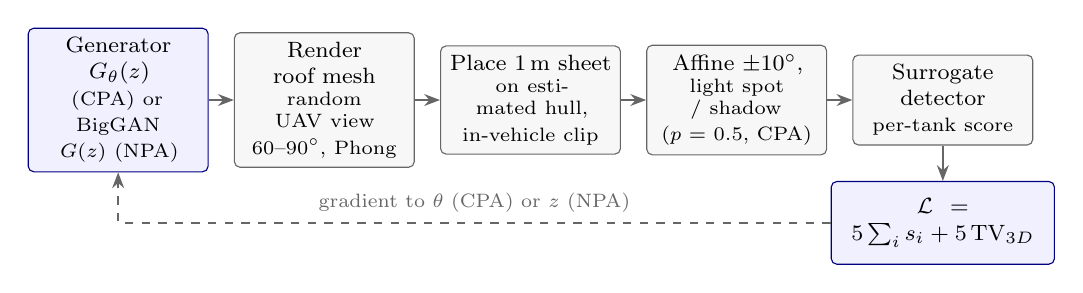
\begin{tikzpicture}[node distance=0.32cm and 0.32cm,
  box/.style={draw=black!60,rounded corners=2pt,fill=black!3,align=center,font=\footnotesize,minimum height=1.05cm,text width=2.05cm},
  hl/.style={box,fill=blue!6,draw=blue!50!black},
  arr/.style={-{Stealth[length=2mm]},thick,black!60}]
\node[hl] (g) {Generator $G_\theta(z)$\\ \scriptsize (CPA) or BigGAN $G(z)$ \scriptsize(NPA)};
\node[box,right=of g] (r) {Render roof mesh\\ \scriptsize random UAV view\\ $60$--$90^\circ$, Phong};
\node[box,right=of r] (p) {Place 1\,m sheet\\ \scriptsize on estimated hull,\\ in-vehicle clip};
\node[box,right=of p] (c) {Affine $\pm10^\circ$,\\ \scriptsize light spot / shadow\\ ($p=0.5$, CPA)};
\node[box,right=of c] (d) {Surrogate\\ detector\\ \scriptsize per-tank score};
\node[hl,below=0.45cm of d,text width=2.6cm] (l) {$\mathcal{L}=5\sum_i s_i+5\,\mathrm{TV}_{3D}$};
\draw[arr] (g)--(r); \draw[arr] (r)--(p); \draw[arr] (p)--(c); \draw[arr] (c)--(d); \draw[arr] (d)--(l);
\draw[arr,dashed] (l.west) -| node[pos=0.25,above,font=\scriptsize]{gradient to $\theta$ (CPA) or $z$ (NPA)} (g.south);
\end{tikzpicture}
\caption{One training step of the 3-D attacks. Only the sheet is rendered; the photograph is real.}
\label{fig:pipeline}
\end{figure}

\paragraph{Patch carrier.} As in CPA, the texture lives on an auxiliary mesh on the roof rather than on the vehicle body: a $32\times32$ vertex grid with $F=1{,}922$ triangular facets (1,938 in the authors' mesh), one RGB colour $C_f$ per facet. The grid is a gentle dome $z=h(1-4x^2)(1-4y^2)$ with $h=6$\,cm on a 1\,m sheet (Figure~\ref{fig:3d}a), approximating a convex turret roof; no 3-D tank model was available, and from 60--90$^\circ$ elevation such a sheet is nearly flat.

\paragraph{Texture generator.} The facet colours are produced by the CPA generator, a 4-layer MLP $G_\theta:\mathbb{R}^{100}\to\mathbb{R}^{3F}$ (widths 256, BatchNorm, LeakyReLU, output $\tfrac12\tanh(0.2\,\cdot)$). In every step
\begin{equation}
C=\frac{1}{K}\sum_{k=1}^{K}G_\theta(z_k)+0.5+\epsilon,\qquad z_k\sim\mathcal{N}(0,I_{100}),\;K=32,\;\epsilon\sim\mathcal{N}(0,0.1^2),
\end{equation}
and only $\theta$ is optimised. Fresh noise in every step forces the texture to work for any noise draw and any small colour error $\epsilon$, an EOT over colour reproduction; sharing one network over all facets favours spatially coherent patterns.

\paragraph{Stochastic weight averaging (SWA).} Every step sees a different view, heading and corruption, so the generator weights keep moving around a minimum instead of settling. SWA \cite{izmailov2018swa} uses the running average of the weights over all steps of the last four of the ten epochs,
\begin{equation}
\bar\theta=\frac{1}{N}\sum_{n=n_0}^{n_0+N-1}\theta_n,
\end{equation}
which lies near the centre of the region the optimiser explores. Such flat minima generalise better: the final texture is good on average over views and corruptions rather than for the last few samples, which is also why CPA uses it to support transfer. The texture is produced by $G_{\bar\theta}$ without the added noise.

\paragraph{Differentiable rendering.} The authors render with PyTorch3D \cite{ravi2020pytorch3d}: a perspective camera with 45$^\circ$ field of view, hard rasterisation (each pixel shows the nearest facet) and Phong shading \cite{phong1975} with the light along the viewing direction. For a camera at $\mathbf{e}$ with rotation $R$, a mesh point $\mathbf{p}$ projects to $u=f\,[R(\mathbf{p}-\mathbf{e})]_{x,y}/[R(\mathbf{p}-\mathbf{e})]_{z}$. Because the geometry is fixed for a given camera, the facet $f(u)$ seen at each pixel and its shading depend only on the camera, so each view is rasterised once and stored. Rendering a texture is then the differentiable gather
\begin{equation}
I(u)=C_{f(u)}\big(k_a+k_d\max(0,\mathbf{n}_u\!\cdot\mathbf{l})\big)+k_s\max(0,\mathbf{r}_u\!\cdot\mathbf{v})^{100},\qquad k_a=0.5,\;k_d=0.3,\;k_s=0.2,
\end{equation}
which is linear in $C$ and gives exactly the gradient $\partial I/\partial C$ of hard rasterisation, at a fraction of the cost.

\paragraph{Viewpoints.} The authors use the true camera pose of every simulator frame; real photographs have none. A bank of 256 views is sampled with elevation $\phi\sim U(60^\circ,90^\circ)$ (90$^\circ$ looks straight down), azimuth $\psi\sim U(0^\circ,360^\circ)$ and distance $d=d_0\,U(0.9,1.1)$, i.e.\ $\mathbf{e}=d(\cos\phi\cos\psi,\cos\phi\sin\psi,\sin\phi)$, and one view is drawn per tank and step. This is EOT over viewpoint: the true angle of each photograph is unknown, so the sheet is optimised to work over the whole range the dataset covers. Testing uses a separately sampled bank. Only the sheet is re-rendered; the photograph keeps its own viewpoint (Figure~\ref{fig:3d}b), an approximation listed in Section~\ref{sec:discussion}.

\paragraph{Printable size and in-vehicle guarantee.} Labels are axis-aligned boxes of size $w\times h$. Modelling the hull as a rectangle of width $W_v$ and length $AW_v$ ($A=1.95$, a main-battle-tank aspect) rotated by $\theta$ gives
\begin{equation}
w=AW_v\cos\theta+W_v\sin\theta,\quad h=AW_v\sin\theta+W_v\cos\theta
\;\;\Rightarrow\;\;
\tan\theta=\frac{A-r}{rA-1},\quad W_v=\frac{w}{A\cos\theta+\sin\theta},
\end{equation}
with $r=w/h$ (if the box is more elongated than $A$, $\theta\in\{0,90^\circ\}$ and $W_v$ is the short side).
The sheet side in pixels is $s=(1\,\text{m}/3.6\,\text{m})\,W_v$ for a 3.6\,m wide hull, so the patch is the same printable 1\,m square in every photograph. A box looks the same for $+\theta$ and $-\theta$, so the sheet is rotated with the hull and multiplied by the mask
\begin{equation}
M(u)=\prod_{\sigma\in\{+1,-1\}}\mathbb{1}\Big[\,\big|[R_{\sigma\theta}(u-c)]_1\big|\le\tfrac{AW_v}{2}-\delta,\;\big|[R_{\sigma\theta}(u-c)]_2\big|\le\tfrac{W_v}{2}-\delta\Big],\qquad\delta=0.05W_v,
\end{equation}
the intersection of both candidate hulls shrunk by a margin, so every patch pixel lies on the vehicle whichever sign is true. The composite is $I'=(1-\alpha M)\odot I+\alpha M\odot I_{\text{sheet}}$, with $\alpha$ the rendered silhouette (Figure~\ref{fig:3d}c, first panel).

\paragraph{Pattern corruptions.} Applied to the \emph{scene}, each with probability 0.5, after a global affine (rotation $\pm10^\circ$, scale 0.9--1.1):
\begin{itemize}
  \item \emph{Light spot} (sun flare): concentric ellipses $E_k$ (axes $1.2r_k\times0.9r_k$, $60^\circ$) centred on a random patch pixel, with radii up to 0.6 of the sheet's side and opacity increasing towards the centre, added to the image, $I'=\min(1,I+\sum_k\beta_k\mathbb{1}_{E_k})$. The addition has an identity Jacobian, so gradients pass unchanged.
  \item \emph{Shadow}: a random quadrilateral $S$ inside the tank box in which the lightness channel of the HLS colour space (hue, lightness, saturation) is halved, $L'=0.5L$ on $S$. This operation is not differentiable in the image library, so a \emph{straight-through estimator} is used: $\tilde I=I+\sg\big(\mathrm{shadow}(I)-I\big)$, where $\sg$ stops the gradient. The forward pass sees the shadowed image and the backward pass treats the shadow as identity, which is reasonable because a shadow mainly rescales brightness.
  \item \emph{Rain and mud} (test only, never seen in training): a random ``liquid'' field $\ell\sim\mathcal{N}(0.65,0.3^2)$ per pixel is blurred ($\sigma=2$\,px) and thresholded at 0.7; rain adds bright drop-shaped highlights along the edges of the resulting blobs, mud replaces the blobs by brown, $I'=I(1-m)+m\,c_{\text{mud}}$ (re-implementation of the \emph{Spatter} transform used by CPA).
\end{itemize}

\paragraph{Loss and optimisation.} For tank $i$ with box $B_i$, let $\Sigma_i$ be the Tank scores of candidates whose centre lies in $B_i$. The per-tank score of the CPA code is
\begin{equation}
s_i=\begin{cases}\operatorname{mean}\{\sigma\in\Sigma_i:\sigma>0.5\} & \text{if }\max\Sigma_i>0.5,\\ \max\Sigma_i & \text{otherwise,}\end{cases}
\end{equation}
so a confidently detected tank has all its confident candidates pushed down (otherwise a neighbouring candidate takes over after NMS), while a weakly detected tank has only its strongest candidate attacked. The loss is
\begin{equation}
\mathcal{L}=5\sum_i s_i+5\,\mathrm{TV}_{3D},\qquad\mathrm{TV}_{3D}=\frac{1}{F}\sum_{(f,g)\text{ adjacent}}\ell_{fg}\,\lVert C_f-C_g\rVert_1,
\end{equation}
where $\ell_{fg}$ is the length of the edge shared by facets $f$ and $g$; this is the 3-D analogue of TV on the mesh. Adam (learning rate 0.01) is used for 10 epochs with two full images per step, and the learning rate is halved whenever the number of tanks scored below 0.5 does not increase over an epoch. Four textures are trained per fold, as in the paper's ablation: \emph{none}, \emph{light}, \emph{shadow} and \emph{light+shadow}.

\begin{figure}[htbp]
\centering
\begin{subfigure}{\linewidth}\centering
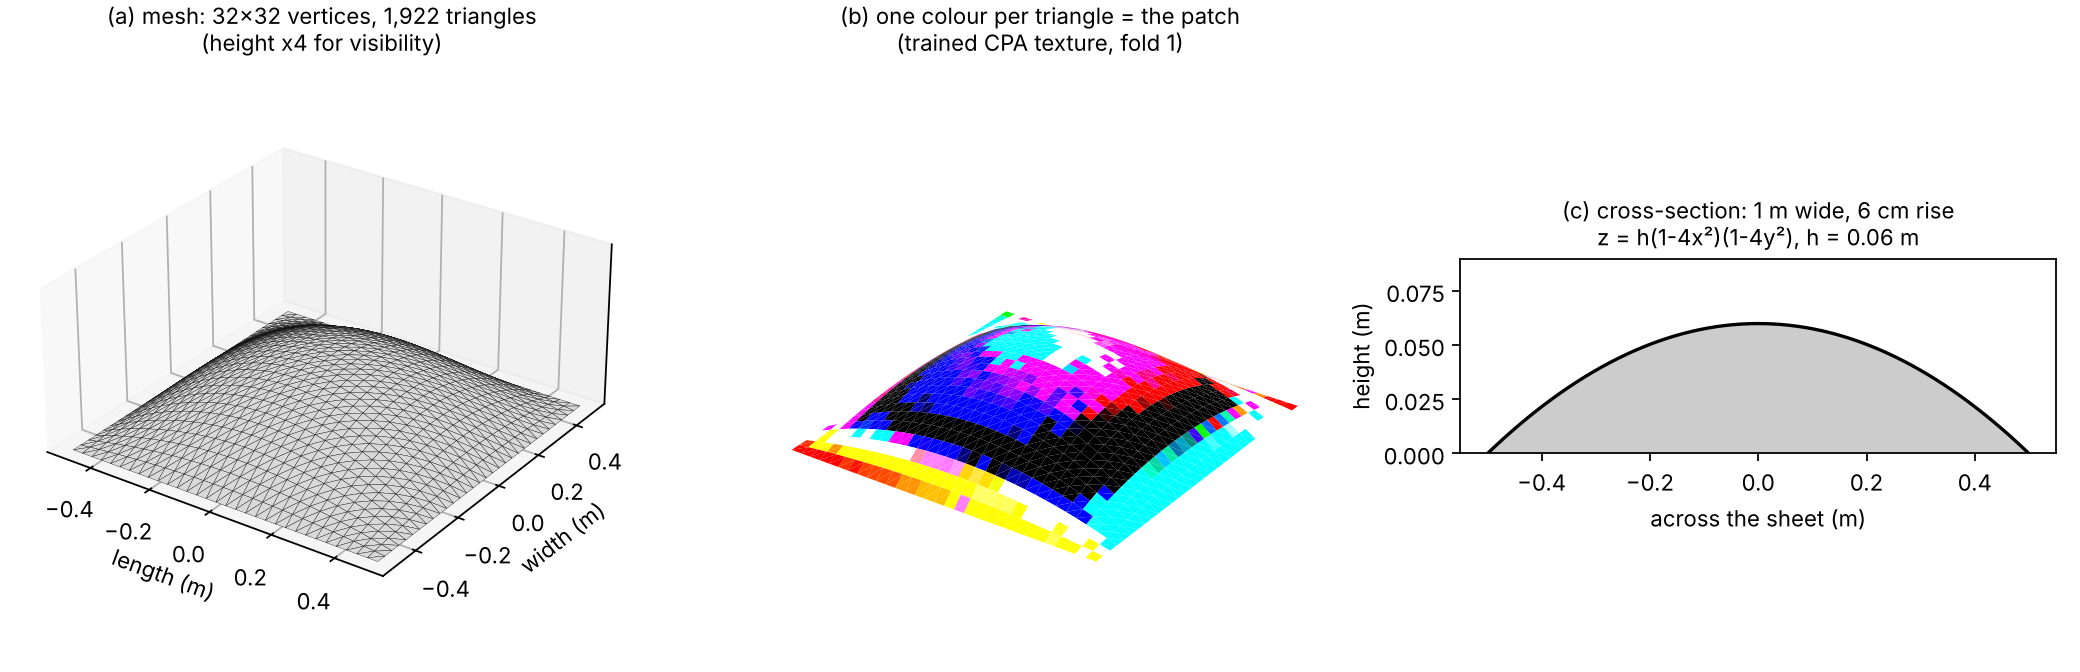
\includegraphics[width=0.92\linewidth]{figures/roof_mesh.png}
\caption{Roof mesh: geometry (height $\times4$), trained CPA texture, cross-section.}
\end{subfigure}\\[4pt]
\begin{subfigure}{0.34\linewidth}\centering
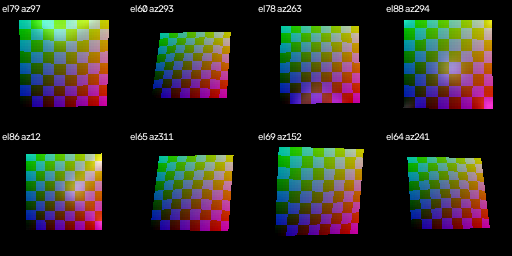
\includegraphics[width=\linewidth]{figures/render_views.png}
\caption{Sheet under 8 sampled UAV views.}
\end{subfigure}\hfill
\begin{subfigure}{0.63\linewidth}\centering
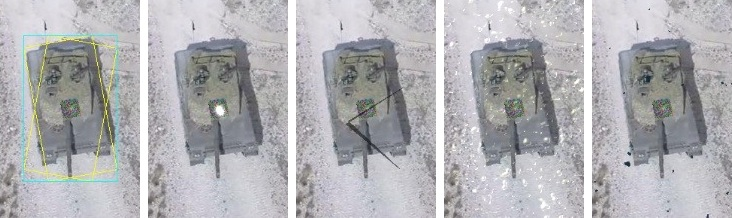
\includegraphics[width=\linewidth]{figures/placement_row_c.jpg}
\caption{On a real tank: placement (yellow: both hull estimates, cyan: label box), light spot, shadow, rain, mud.}
\end{subfigure}
\caption{Components of the 3-D attack.}
\label{fig:3d}
\end{figure}

\subsection{Stage 3: naturalistic patches}\label{sec:npa}
\paragraph{NPA.} BigGAN-128 \cite{brock2019} is a pretrained generator $G(z,y)$ that maps a latent vector $z\in\mathbb{R}^{120}$ and an ImageNet class $y$ to a $128\times128$ image. The patch is $P=(G(z,y)+1)/2$, mapped onto the 1\,m sheet by per-pixel texture coordinates (UV mapping) so that it is rendered, placed and evaluated exactly like the CPA texture. Only $z$ is optimised:
\begin{equation}
\min_z\;\frac{1}{N}\sum_i\max_{a\in B_i}s_a+0.1\,\mathrm{TV}(P),\qquad z\leftarrow\operatorname{clip}(z,-\tau,\tau)\text{ after every step},
\end{equation}
with Adam (learning rate 0.005, $\beta=(0.5,0.999)$) for 20 epochs of batch 4. Because the patch is always an output of a generator trained on photographs, it should stay on the manifold of natural images; the clamp $\tau$ is the paper's realism control. The paper's class (259, a dog) and $\tau=10$ were tested with $\tau=4,2$ and two scene classes with terrain colours (958, hay; 977, sandbar). The paper's no-GAN baseline optimises the $128\times128$ pixels directly.

\paragraph{Measuring naturalness.} No user study was possible, so the main proxy is the share of saturated pixels,
\begin{equation}
\mathrm{sat}(P)=\frac{1}{|U|}\sum_{u\in U}\mathbb{1}\big[\exists c:\;P_c(u)<0.03\;\lor\;P_c(u)>0.97\big],
\end{equation}
checked by eye on image sheets. Gradient attacks drive pixels to the bounds of $[0,1]$ because the loss keeps decreasing until the box constraint stops them, whereas natural photographs rarely clip; all start images have $\mathrm{sat}<1.5\,\%$.

\paragraph{Remedies for lost naturalness.} The clamp alone did not keep patches natural (Section~\ref{sec:res-npa}), so four remedies were tested, all with class 977 and $\tau=3$:
\begin{itemize}
  \item \emph{Latent on the sphere.} For $z\sim\mathcal{N}(0,I_d)$, $\mathbb{E}\lVert z\rVert^2=d$ and $\mathrm{Var}\lVert z\rVert^2=2d$, so $\lVert z\rVert$ concentrates at $\sqrt d\approx11$ with standard deviation $\approx0.7$; the generator has only seen latents on this thin shell. A box $[-\tau,\tau]^d$ still allows $\lVert z\rVert$ up to $\tau\sqrt d$, so after every step $z\leftarrow\sqrt d\,z/\lVert z\rVert$ keeps the length typical and lets only the direction change.
  \item \emph{Coarse latent.} BigGAN splits $z$ into six chunks of 20; chunk 0 sets the $4\times4$ layout and chunks 1--5 condition the five upsampling blocks. Optimising only chunks 0--2 changes layout and colour but not fine texture.
  \item \emph{Saturation penalty} $\;\mathcal{R}=\operatorname{mean}_u\max(0,|P(u)-0.5|-0.45)/0.05$, added to the loss, which is zero for pixel values in $[0.05,0.95]$.
  \item \emph{Naturalness-budget early stop.} The patch $P_e$ is saved after every epoch and the last one within a saturation budget $S$ is kept, $e^*=\max\{e:\mathrm{sat}(P_e)\le S\}$ ($S=20\,\%$; the start image if no epoch qualifies). Since this only selects among saved epochs, varying $S$ traces a realism--attack curve along the same training runs.
\end{itemize}

\paragraph{Camouflage (AdvCaT).} A natural-by-construction alternative \cite{hu2023advcat}: the patch may only use $C=4$ palette colours $\kappa_c$ (a woodland camouflage palette, or the four k-means colours of tank pixels in the training images). Each colour owns 15 movable control points $b_{cj}$, and a pixel's colour probabilities come from a soft Voronoi map,
\begin{equation}
p_c(u)=\frac{\sum_j\exp(-\lVert u-b_{cj}\rVert/\beta)}{\sum_{c'}\sum_j\exp(-\lVert u-b_{c'j}\rVert/\beta)},\qquad\beta=1\text{ px},
\end{equation}
smoothed by a $3\times3$ mean filter, which produces blob-shaped regions like printed camouflage. Choosing one colour per pixel is discrete, so training uses the Gumbel-softmax relaxation \cite{jang2017gumbel},
\begin{equation}
P(u)=\sum_c\pi_c(u)\,\kappa_c,\qquad\pi(u)=\operatorname{softmax}\big((\log p(u)+g(u))/\tau_g\big),\quad g=-\log(-\log U),\;\tau_g=0.3,
\end{equation}
where $U=0.7\,U_{\text{train}}+0.3\,U_{\text{fixed}}$ mixes optimised and fixed uniform noise, so the optimiser can bias which colour wins in ambiguous regions while keeping some randomness. The control points (Adam, $10^{-3}$) and $U_{\text{train}}$ ($10^{-2}$) are trained with the NPA detection loss and a concentration term that keeps same-colour points close; testing and printing use the hard choice $\arg\max_c p_c(u)$. Sheets of 1\,m and 3\,m were tested.

\subsection{Transfer metrics and experiments}
Every 3-D attack is also trained with each black-box detector as surrogate, giving a $4\times4$ matrix of margins $m_{jk}$ (trained on $j$, tested on $k$). The white-box and black-box means are $W=\frac14\sum_j m_{jj}$ and $B=\frac1{12}\sum_{j\ne k}m_{jk}$, and $B/W$ is the share of the effect that transfers. Table~\ref{tab:experiments} lists all experiments; every variant is trained once per fold and all are evaluated on the same held-out tanks, views and corruption draws.

\begin{table}[htbp]
\centering\small
\caption{Experiments. All use the 5 photo-grouped folds and the same held-out tanks.}
\label{tab:experiments}
\begin{tabularx}{\linewidth}{@{}p{3.1cm}Yp{4.3cm}@{}}
\toprule
Experiment & Variants & Question \\
\midrule
Detectors & YOLOv8s 960\,px; 1280\,px; DOTA initialisation; YOLOv8m, YOLO11s, RT-DETR-l & Baseline; black-box targets \\
2-D patches & EOT; CPA light / shadow / light+shadow; Tank and Aircraft & Pattern vs occlusion; per-class effect \\
3-D CPA & none / light / shadow / light+shadow, 1\,m sheet & CPA ablation on real photographs \\
Transfer matrix & cpa\_none, cpa\_ls, natural NPA, trained on each of the 4 detectors & White-box vs black-box \\
CPA ablations & sheet 1 / 1.5 / 2\,m; 2 seeds; corruption $p=1$; fixed view per tank & Why no CPA gain? \\
NPA & class 259 / 958 / 977; $\tau=10,4,2$; pixel baseline & Paper's realism control \\
Naturalness & sphere, coarse latent, saturation penalty, early stop ($S=5$--$100\,\%$); AdvCaT 1\,m, 3\,m & Natural and adversarial? \\
\bottomrule
\end{tabularx}
\end{table}

\subsection{Implementation checks}
Three implementation issues were found by cross-checking and fixed before the reported runs: Ultralytics reads NumPy arrays as BGR, and passing RGB arrays had cut the detected tanks from 244 to 30; the evaluator had run at 640\,px for detectors trained at 960\,px; and for RT-DETR the attack had read scores from the post-processed top-$k$ output, which gave wrong gradients, so scores are now read per class from the decoder, verified against the detector's own predictions, and those patches were retrained.

%=====================================================================
\section{Results and discussion}\label{sec:results}

The results are presented in the order of the project stages: the detector baseline (Stage 0), the 2-D patches (Stage 1: pilot, cross-validated study, Aircraft, and the effect on detection metrics), the 3-D CPA patch (Stage 2) with its transfer and ablation studies, and the naturalistic patches (Stage 3). Detailed per-detector tables are in Appendix~\ref{app:tables}.

\subsection{Stage 0: detector baseline}\label{sec:res-det}
\paragraph{Development.} Table~\ref{tab:devruns} lists the training runs that led to the final detector recipe.

\begin{table}[htbp]
\centering\small
\caption{Detector development runs (YOLOv8s, COCO initialisation). Validation mAP50 is the best epoch on the stated validation data; ``test'' is the official 16-image test split.}
\label{tab:devruns}
\setlength{\tabcolsep}{3.5pt}
\begin{tabularx}{\linewidth}{@{}p{3.4cm}p{3.6cm}Ycc@{}}
\toprule
Run & Validation data & Settings & val.\ mAP50 (epoch) & test mAP50 \\
\midrule
Initial baseline & official Validation, 16 images & 640\,px, batch 32 & 0.555 (11 of 31) & -- \\
File-level dev split & 12\,\% of training files & 960\,px, rare classes oversampled & 0.86 & 0.20 \\
Photo-level dev split & 11 held-out photographs & 960\,px, oversampled & 0.255 (2 of 42) & 0.480 \\
\quad + frozen backbone & same & first 10 layers frozen & 0.261 (7 of 17) & -- \\
\quad no oversampling & same & -- & 0.257 (3 of 13) & -- \\
\quad frozen, no oversampling & same & -- & 0.269 (3 of 13) & -- \\
\midrule
Final, per CV fold & held-out fold (16--20 photos) & 960\,px, frozen, oversampled, $\le$15 epochs & $0.195\pm0.037$ & $0.436\pm0.028$ \\
\bottomrule
\end{tabularx}
\end{table}

Three conclusions follow. First, the 16-image official validation split is too small to select a checkpoint: the score jumps between epochs, and the reported 0.555 does not carry over to unseen photographs. Second, the file-level split leaked (0.86 versus 0.20 on the test split), which led to the photo-grouped protocol. Third, once leakage is removed, freezing the backbone and removing oversampling change validation mAP50 by less than 0.015 and the best epoch is always early (2--7): the ceiling is set by the number of distinct photographs, not by the hyper-parameters. The frozen backbone with early stopping was kept because it overfits least.

\paragraph{Final baseline.} Table~\ref{tab:det} gives precision, recall and AP per class for the five cross-validated detectors, and Figure~\ref{fig:det} shows the training curves and evaluation plots of one fold.

\begin{table}[htbp]
\centering\small
\caption{Clean baseline of YOLOv8s (960\,px), mean $\pm$ s.d.\ over the 5 fold detectors.}
\label{tab:det}
\setlength{\tabcolsep}{3.5pt}
\begin{tabular}{@{}lcccccccc@{}}
\toprule
 & \multicolumn{4}{c}{Held-out photographs (validation)} & \multicolumn{4}{c}{Official test split} \\
\cmidrule(lr){2-5}\cmidrule(lr){6-9}
Class & P & R & AP50 & AP50-95 & P & R & AP50 & AP50-95 \\
\midrule
Aircraft & 0.50 & 0.32 & $0.29\pm0.11$ & 0.14 & 0.65 & 0.63 & $0.64\pm0.06$ & 0.39 \\
Building & 0.36 & 0.33 & $0.25\pm0.09$ & 0.14 & 0.48 & 0.61 & $0.53\pm0.11$ & 0.32 \\
Military Truck & 0.18 & 0.09 & $0.06\pm0.07$ & 0.03 & 0.25 & 0.07 & $0.07\pm0.01$ & 0.05 \\
Tank & 0.41 & 0.20 & $0.18\pm0.19$ & 0.12 & 0.64 & 0.42 & $0.50\pm0.13$ & 0.22 \\
\midrule
All (mAP) & 0.36 & 0.24 & $0.195\pm0.037$ & 0.107 & 0.51 & 0.43 & $0.436\pm0.028$ & 0.245 \\
\bottomrule
\end{tabular}
\end{table}

\begin{figure}[htbp]
\centering
\begin{subfigure}{0.62\linewidth}\centering
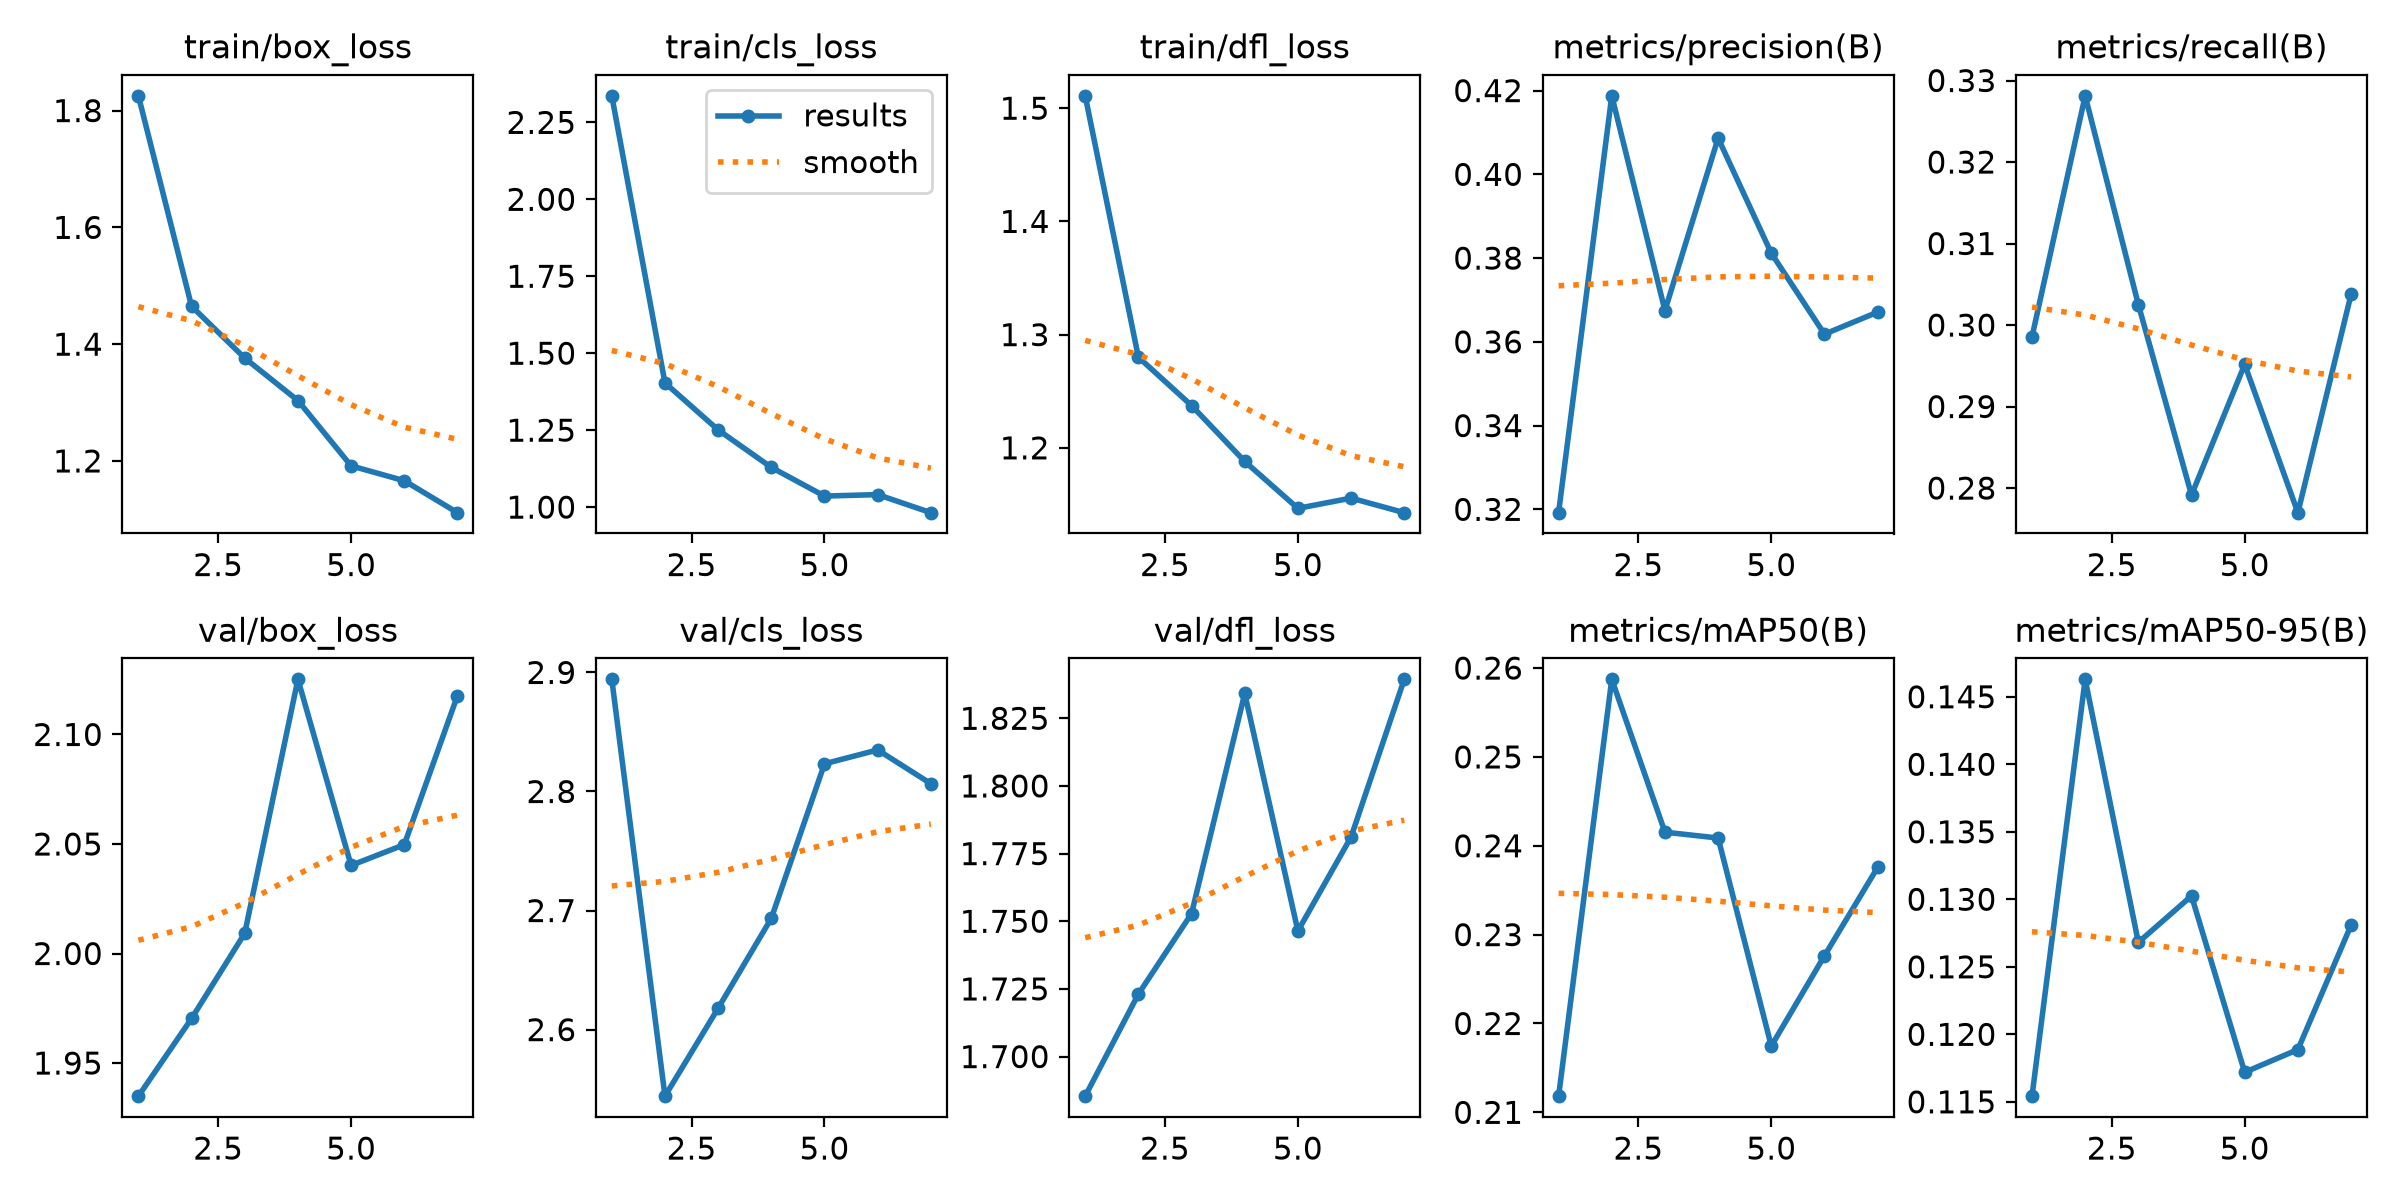
\includegraphics[width=\linewidth]{figures/det_train_curves.png}
\caption{Training losses and validation metrics per epoch.}
\end{subfigure}\hfill
\begin{subfigure}{0.36\linewidth}\centering
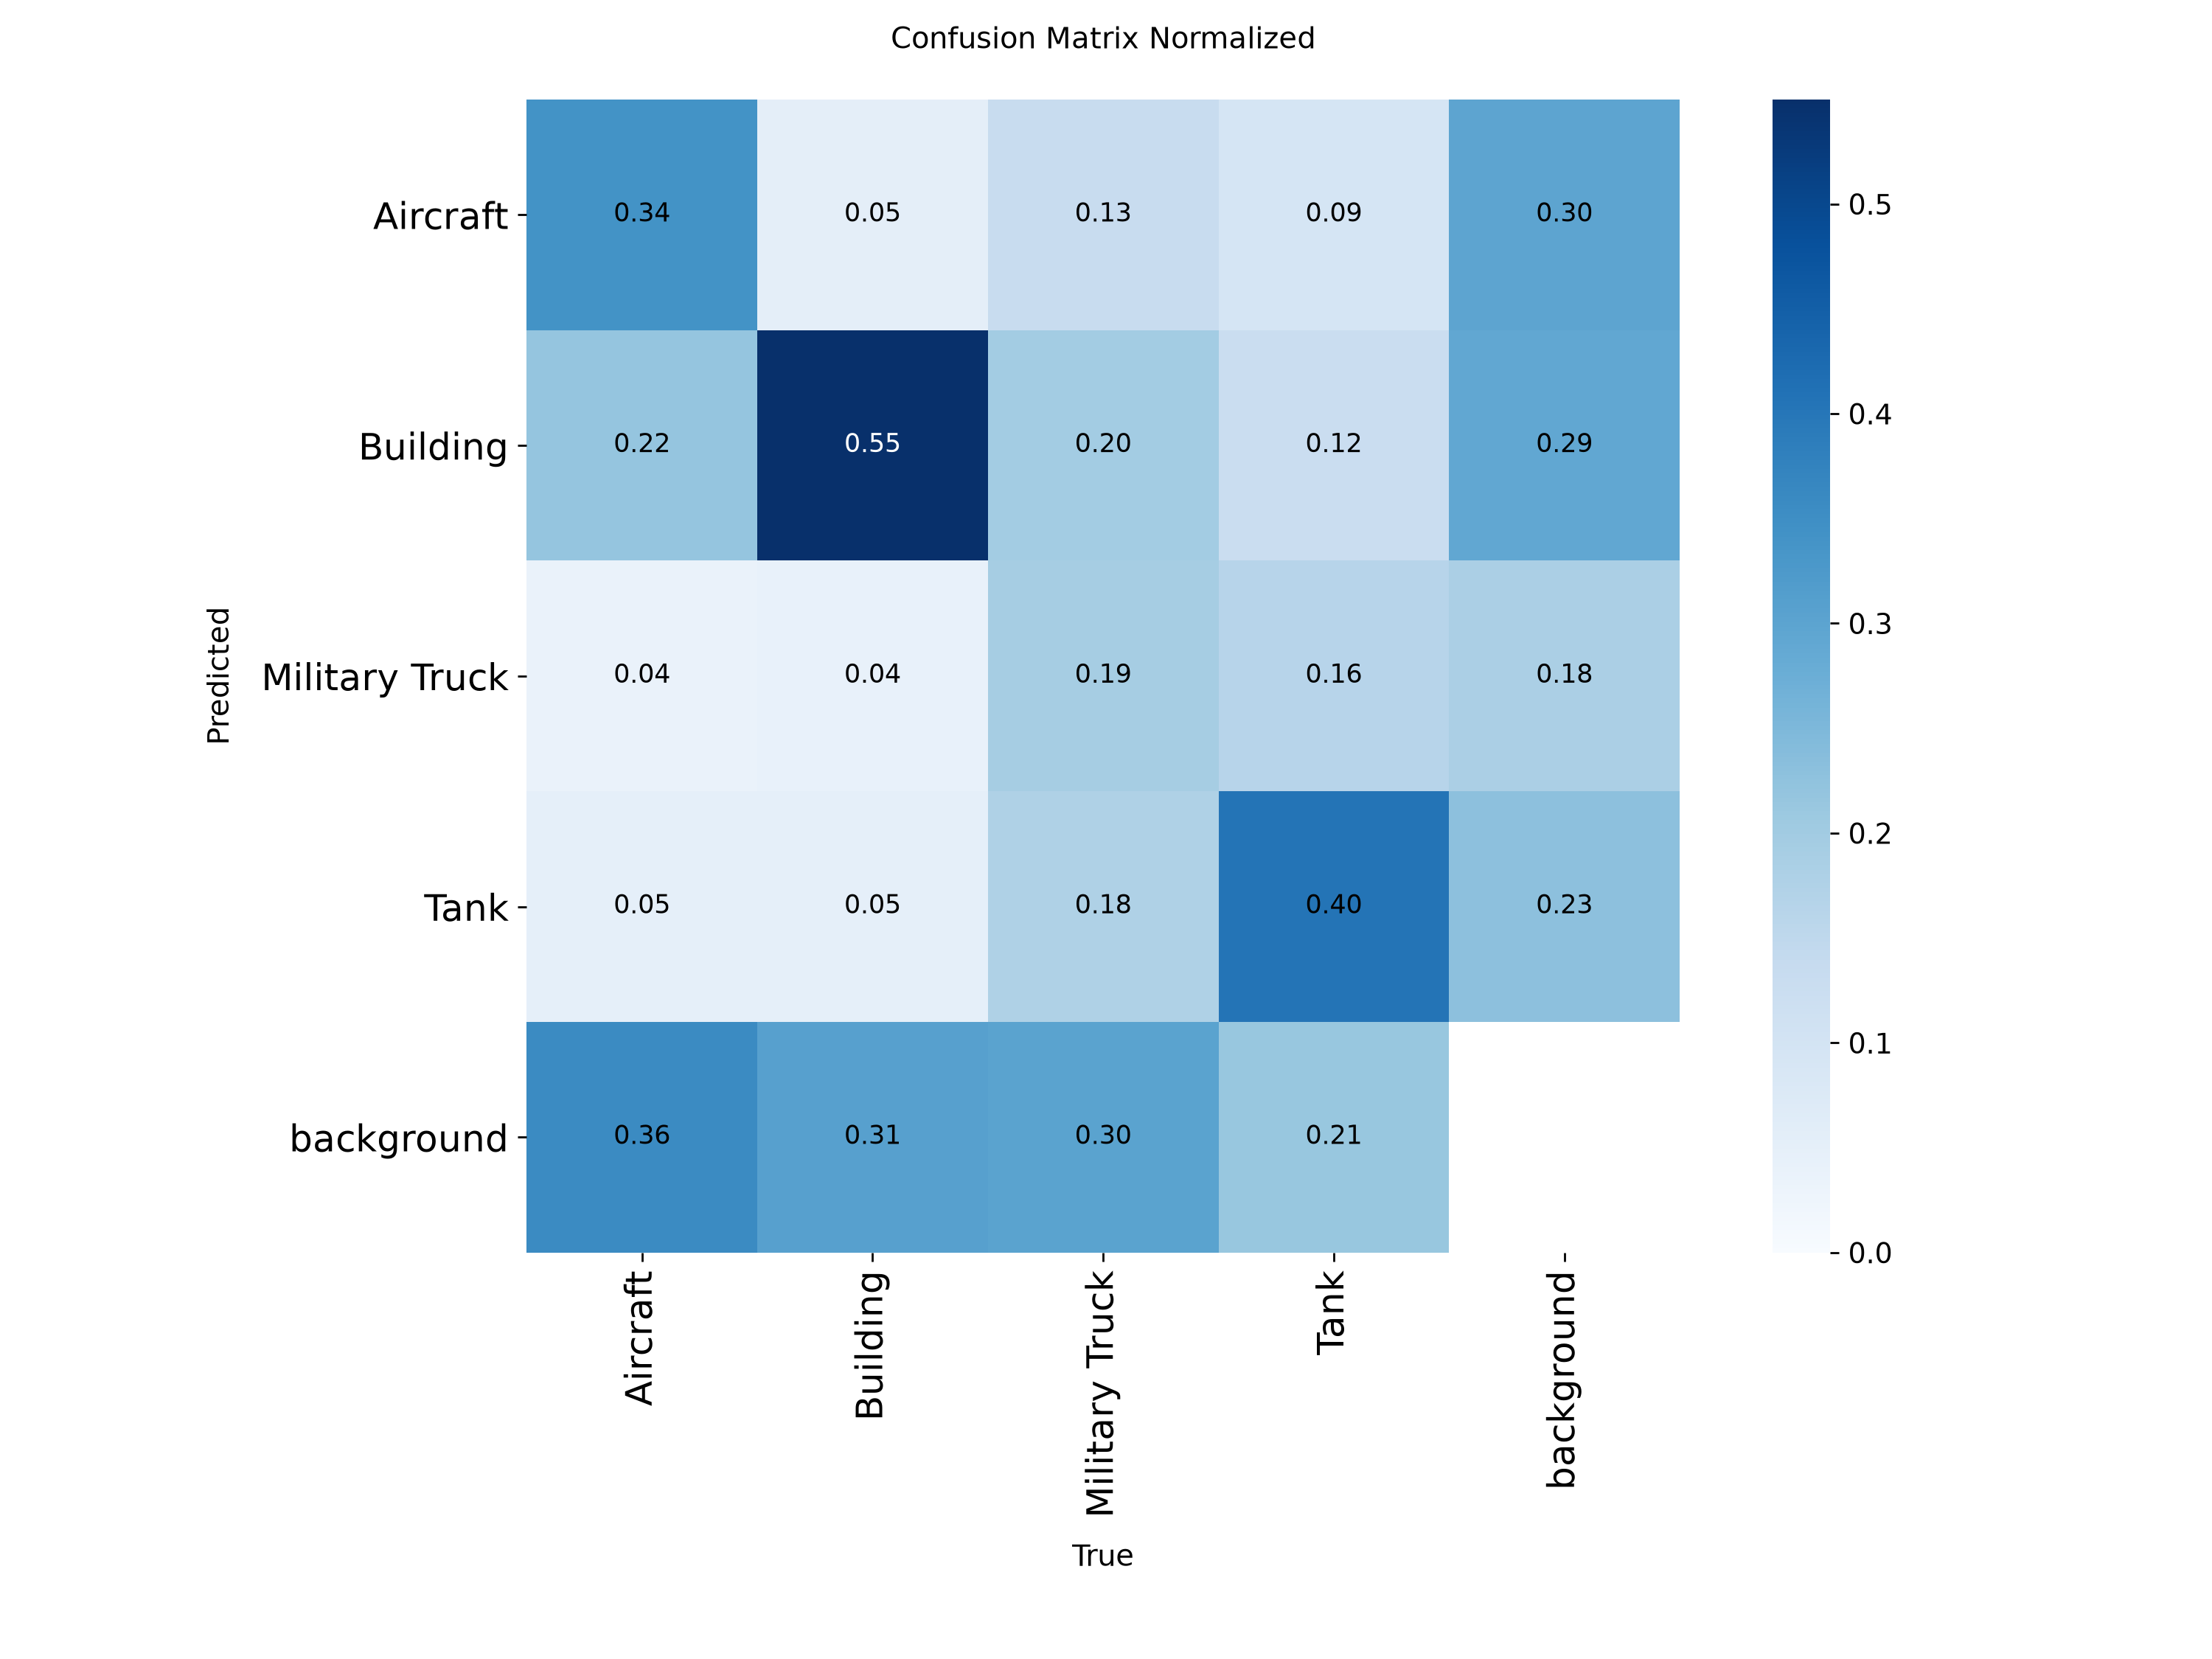
\includegraphics[width=\linewidth]{figures/det_cm_val.png}
\caption{Normalised confusion matrix, held-out photographs.}
\end{subfigure}\\[3pt]
\begin{subfigure}{0.45\linewidth}\centering
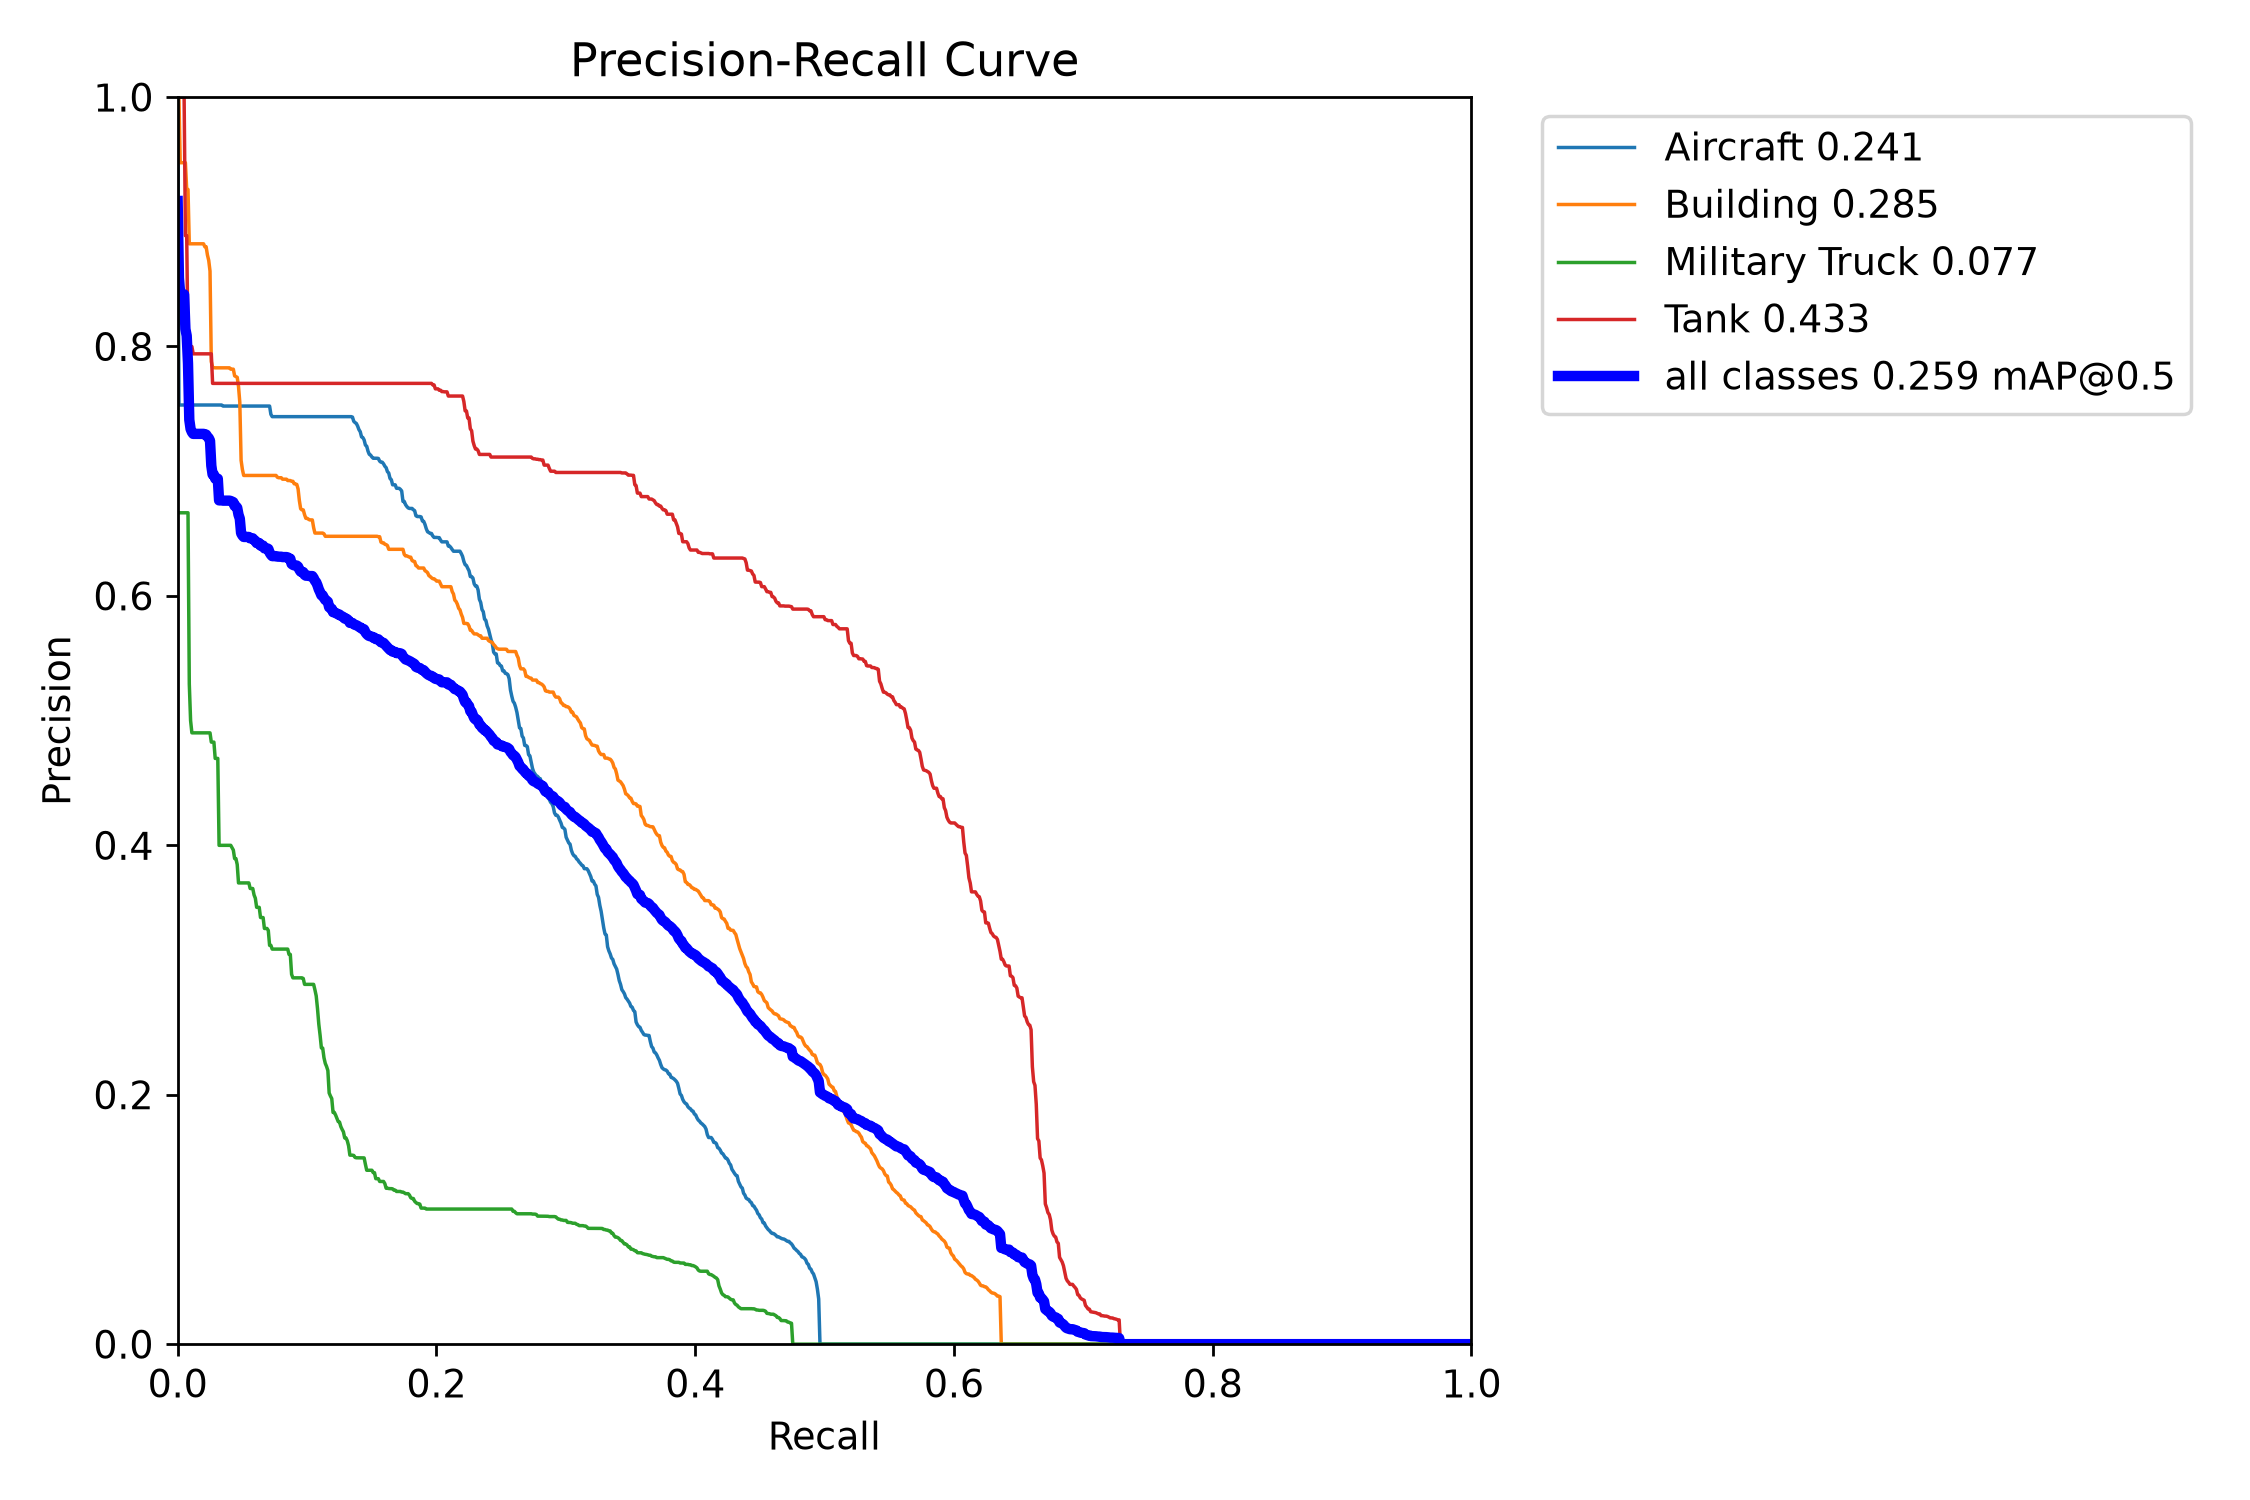
\includegraphics[width=\linewidth]{figures/det_pr_val.png}
\caption{Precision--recall curves, held-out photographs.}
\end{subfigure}\hspace{0.04\linewidth}
\begin{subfigure}{0.45\linewidth}\centering
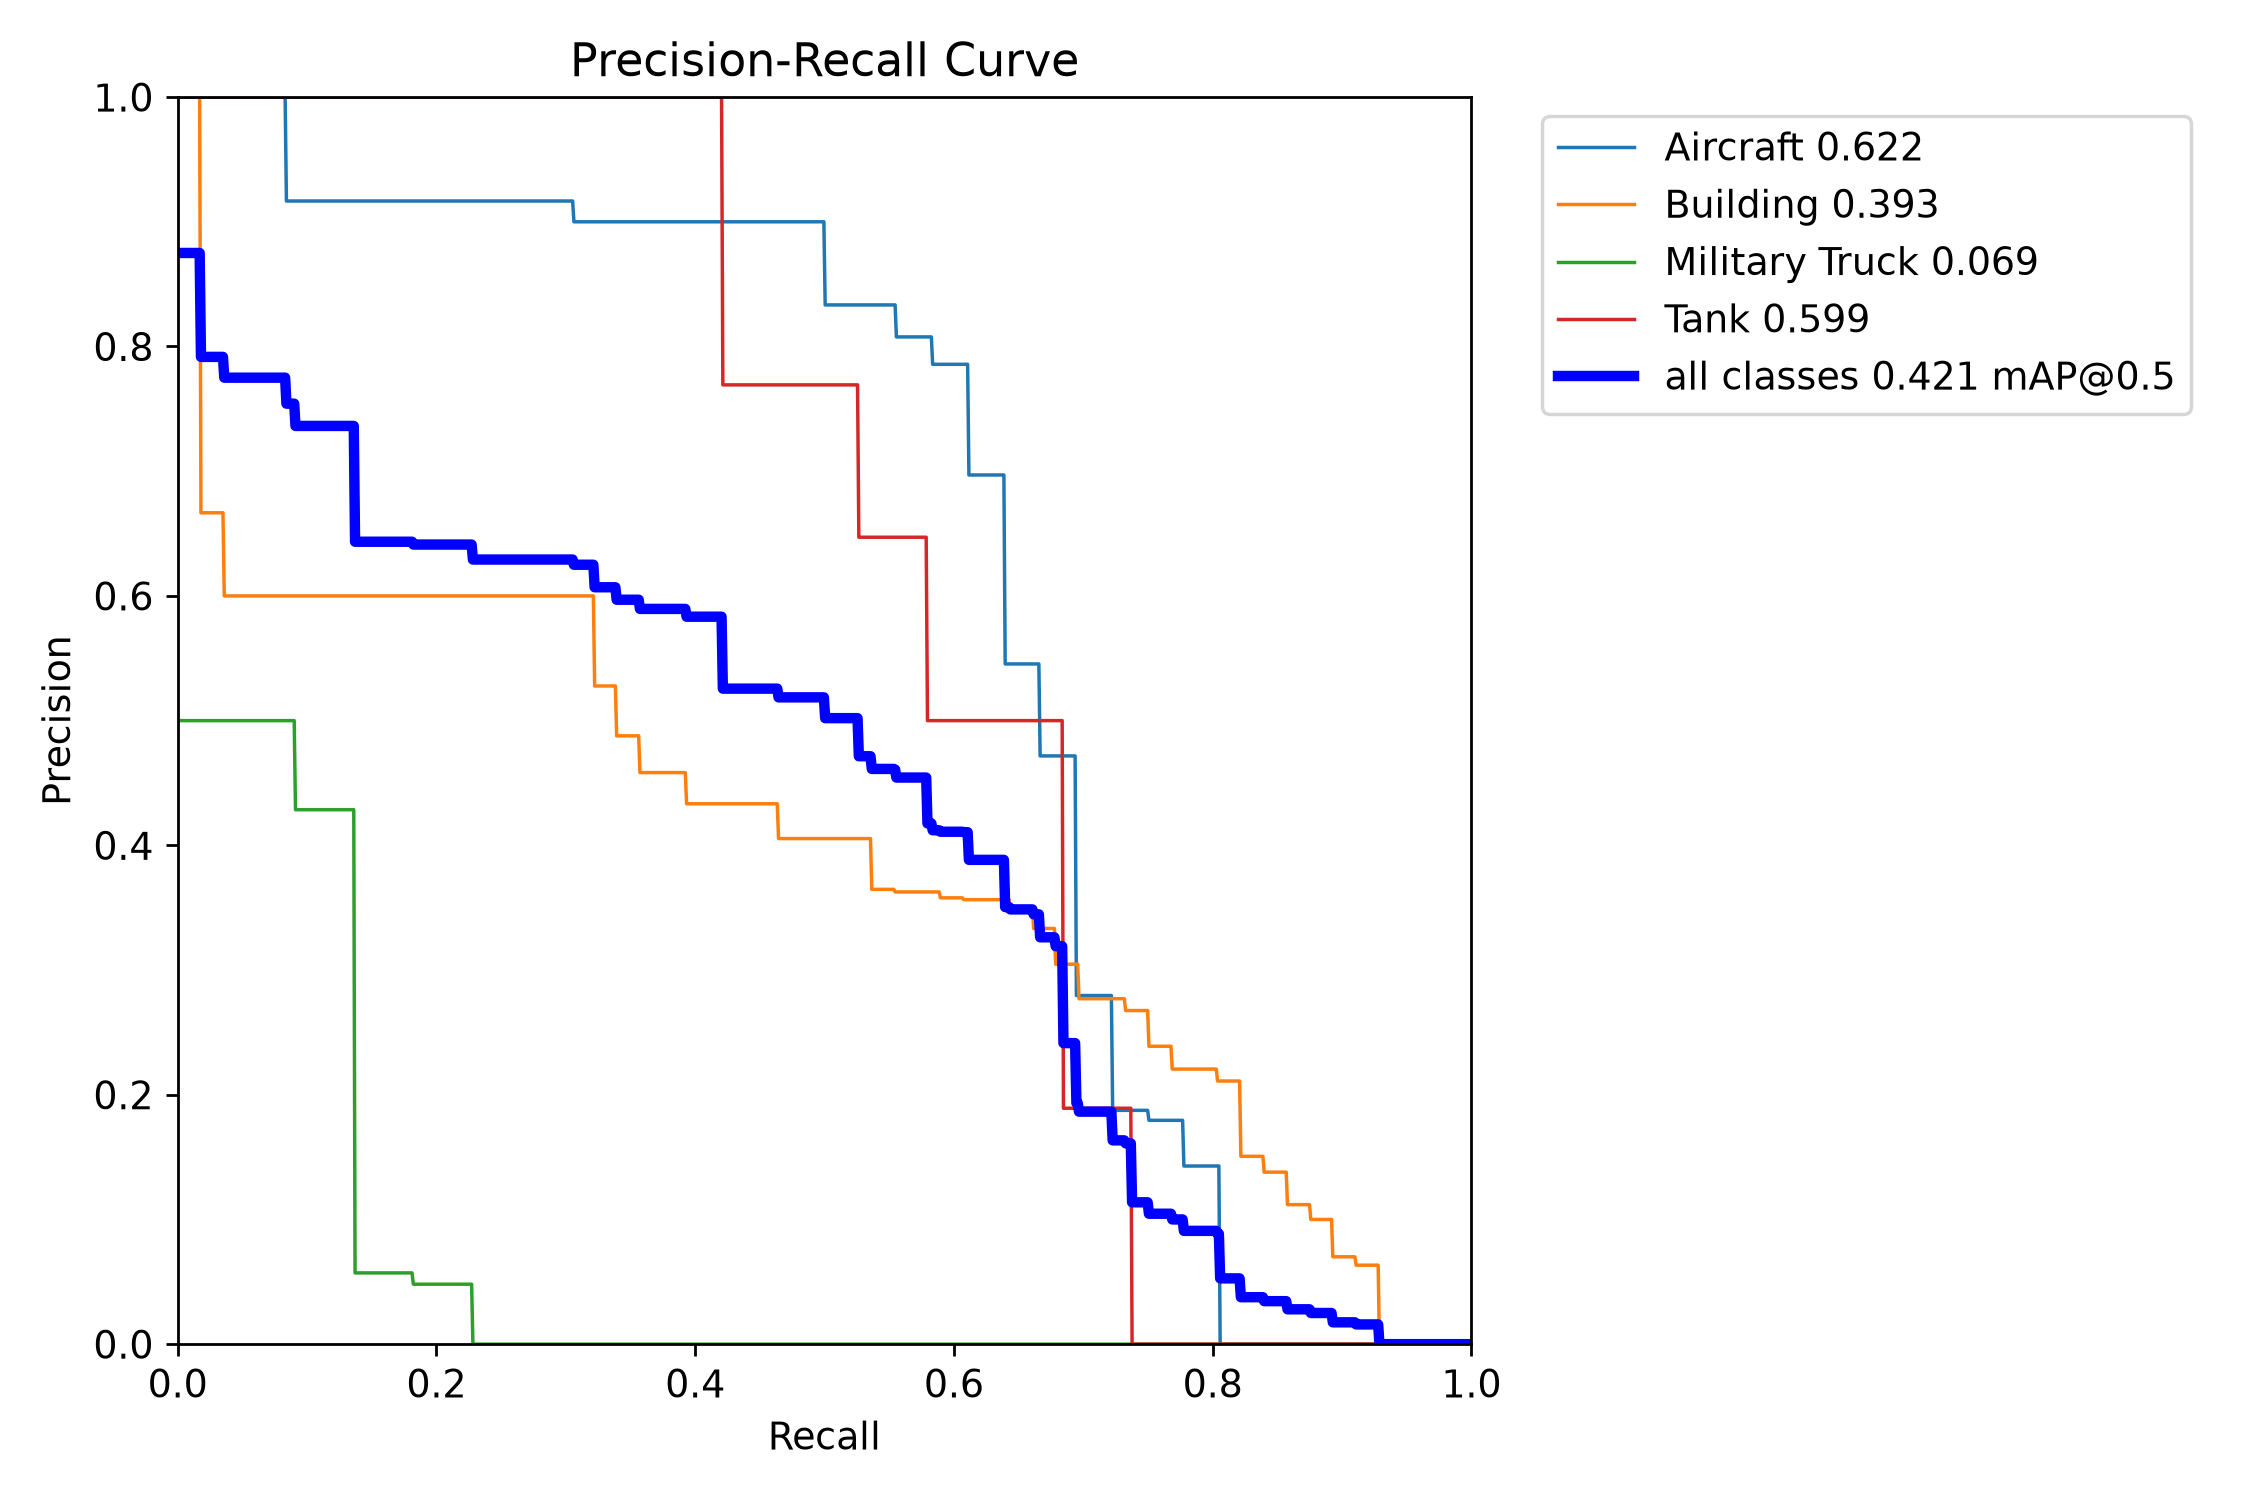
\includegraphics[width=\linewidth]{figures/det_pr_test.png}
\caption{Precision--recall curves, official test split.}
\end{subfigure}
\caption{YOLOv8s detector of fold 1.}
\label{fig:det}
\end{figure}

On photographs it never saw, the detector reaches mAP50 0.20 with large fold-to-fold variation (Tank AP50 from 0.03 to 0.43 between folds); the official test split, whose photographs resemble the training pool more closely, gives 0.44. Validation losses rise after a few epochs while training losses keep falling (Figure~\ref{fig:det}a), the signature of memorising about 70 photographs. In the fold-1 confusion matrix (Figure~\ref{fig:det}b) Military Truck is recognised in only 19\,\% of cases and is otherwise split between background (30\,\%), Building, Tank and Aircraft; 40\,\% of tanks are recognised, 21\,\% are missed and 16\,\% are labelled Military Truck. The two vehicle classes are hard to separate from above, which is another reason to attack Tank, the better-learnt of the two.

\paragraph{Detector variants and black-box detectors.} Table~\ref{tab:detvar} compares the variants trained on the same folds.

\begin{table}[htbp]
\centering\small
\caption{Held-out AP50 per class (mean over 5 folds) of all detectors; official-test mAP50 where it was evaluated.}
\label{tab:detvar}
\setlength{\tabcolsep}{4pt}
\begin{tabular}{@{}lcccccc@{}}
\toprule
Detector & Aircraft & Building & Mil.\ Truck & Tank & mAP50 & test mAP50 \\
\midrule
YOLOv8s, 960\,px (surrogate) & 0.288 & 0.249 & 0.060 & 0.180 & 0.195 & 0.436 \\
YOLOv8s, 1280\,px & 0.323 & 0.281 & 0.062 & 0.163 & 0.208 & 0.439 \\
YOLOv8s, DOTA init., 1280\,px & 0.410 & 0.277 & 0.079 & 0.156 & 0.230 & 0.438 \\
\midrule
YOLOv8m (black-box) & 0.332 & 0.265 & 0.069 & 0.199 & 0.216 & -- \\
YOLO11s (black-box) & 0.341 & 0.298 & 0.089 & 0.196 & 0.231 & -- \\
RT-DETR-l (black-box) & 0.383 & 0.356 & 0.099 & 0.225 & 0.266 & -- \\
\bottomrule
\end{tabular}
\end{table}

A larger input and aerial pre-training raise Aircraft AP (official test $0.64\to0.67$ and $0.77$) but not Tank AP, and all six detectors are within 0.08 mAP50 of each other: the data, not the architecture, limits accuracy. DOTA initialisation was therefore used only for the Aircraft attack. RT-DETR-l is the strongest detector, which makes it the most demanding black-box target.

\subsection{Stage 1: pilot study}\label{sec:res-pilot}
Before cross-validation, EOT patches were trained on the photo-level development split and evaluated on its 11 held-out photographs; only 2 of them contain tanks (244 detected tank instances). Table~\ref{tab:pilot} shows the effect of patch size and of patch corruptions.

\begin{table}[htbp]
\centering\small
\caption{Pilot on 2 held-out tank photographs (244 instances, confidence 0.25): share of detected tanks hidden. Left: EOT patch of three widths; right: EOT vs a patch trained with corruptions (width 0.3) under each test condition.}
\label{tab:pilot}
\setlength{\tabcolsep}{4pt}
\begin{tabular}{@{}lccc@{\hspace{1.2em}}lccc@{}}
\toprule
Width & patch & gray & noise & Condition & EOT & CPA-style & gray \\
\midrule
$0.3w$ & 0.56 & 0.33 & 0.23 & none & 0.56 & 0.54 & 0.33 \\
$0.5w$ & 0.96 & 0.69 & 0.41 & light & 0.47 & 0.45 & 0.25 \\
$0.7w$ & 0.98 & 0.96 & 0.78 & shadow & 0.43 & 0.51 & 0.30 \\
 & & & & rain & 0.53 & 0.52 & 0.27 \\
 & & & & mud & 0.25 & 0.47 & 0.17 \\
\bottomrule
\end{tabular}
\end{table}

The pattern clearly beats occlusion at widths 0.3 and 0.5, but at 0.7 a gray square alone hides 96\,\% of the tanks, so a large patch proves nothing about the pattern; 0.4 was chosen for the main 2-D study. The corruption-trained patch looked much more robust to mud (0.47 versus 0.25). These numbers come from only two scenes, however, so the instances are not independent and the apparent CPA advantage could be specific to those scenes; this is what motivated the photo-grouped cross-validation.

\subsection{Stage 1: cross-validated 2-D study}\label{sec:res-2d}
Pooled over the five folds, 185 tanks in 17 held-out photographs were detected before patching (confidence 0.25). A first run with 20 patch epochs and one seed suggested that CPA beats EOT under corruption by about 0.10 (Table~\ref{tab:2dconv}); its training logs, however, showed the patch loss still falling. Rerunning with 80 epochs and three seeds showed the confidence drop on training crops rising from 0.114 (epoch 10) to 0.198 (epoch 30) and then plateauing at 0.18--0.22. EOT gained most from the longer training and the CPA lead shrank to 0.06, no longer significant after correction.

\begin{table}[htbp]
\centering\small
\caption{2-D Tank patches (width $0.4w$, confidence 0.25): margin over the best control after 20 epochs (one seed) and after 80 epochs (three seeds), and the paired CPA light+shadow $-$ EOT difference under corruption.}
\label{tab:2dconv}
\setlength{\tabcolsep}{4pt}
\begin{tabular}{@{}lcccc@{}}
\toprule
 & \multicolumn{2}{c}{20 epochs} & \multicolumn{2}{c}{80 epochs} \\
\cmidrule(lr){2-3}\cmidrule(lr){4-5}
 & no corruption & corruption avg & no corruption & corruption avg \\
\midrule
EOT & $+0.270$ & $+0.188$ & $+0.319$ & $+0.280$ \\
CPA light & $+0.227$ & $+0.215$ & $+0.297$ & $+0.289$ \\
CPA shadow & $+0.330$ & $+0.297$ & $+0.366$ & $+0.314$ \\
CPA light+shadow & $+0.335$ & $+0.291$ & $+0.378$ & $+0.340$ \\
\midrule
CPA light+shadow $-$ EOT & \multicolumn{2}{c}{$+0.103$ (corr.), $p=0.063$, Holm 0.79} & \multicolumn{2}{c}{$+0.060$ (corr.), $p=0.015$, Holm 0.21} \\
\bottomrule
\end{tabular}
\end{table}

Table~\ref{tab:2d} gives the final 80-epoch results with intervals, and Table~\ref{tab:2dcond} every test condition. Every patch hides about 0.3 more tanks than a control of the same size and place, with photo-level intervals well above zero, and the margin survives rain and mud, which were never used in training. Mud lowers the raw success of every patch the most (0.55--0.62) but the margin over the control stays positive, because mud also lowers the control. Across seeds the margin varies by at most $\pm0.06$ (EOT: $+0.35$, $+0.31$, $+0.30$; CPA shadow: $+0.42$, $+0.30$, $+0.37$), and across folds from $+0.21$ to $+0.67$, so differences between methods smaller than about 0.06 cannot be distinguished. Figures~\ref{fig:2d} and~\ref{fig:2dex} show the patches and examples.

\begin{table}[htbp]
\centering\small
\caption{2-D Tank patches after 80 epochs (confidence 0.25, 3 seeds): share of detected tanks hidden and margin over the best control [95\,\% photo-level interval].}
\label{tab:2d}
\setlength{\tabcolsep}{4pt}
\begin{tabular}{@{}lcccc@{}}
\toprule
 & \multicolumn{2}{c}{No corruption} & \multicolumn{2}{c}{Light/shadow/rain/mud (avg)} \\
\cmidrule(lr){2-3}\cmidrule(lr){4-5}
Method & hidden & margin & hidden & margin \\
\midrule
EOT & 0.816 & $+0.319$ \ci{$+0.21$}{$+0.41$} & 0.725 & $+0.280$ \ci{$+0.16$}{$+0.40$} \\
CPA light & 0.795 & $+0.297$ \ci{$+0.17$}{$+0.41$} & 0.733 & $+0.289$ \ci{$+0.16$}{$+0.41$} \\
CPA shadow & 0.863 & $+0.366$ \ci{$+0.26$}{$+0.45$} & 0.758 & $+0.314$ \ci{$+0.20$}{$+0.42$} \\
CPA light+shadow & 0.876 & $+0.378$ \ci{$+0.28$}{$+0.47$} & 0.785 & $+0.340$ \ci{$+0.23$}{$+0.45$} \\
\midrule
\textit{best control} & 0.497 & & 0.445 & \\
\bottomrule
\end{tabular}
\end{table}

\begin{table}[htbp]
\centering\small
\caption{2-D Tank patches, every test condition: hidden share / margin over the best control. $^\ast$ corruption used in that method's training.}
\label{tab:2dcond}
\setlength{\tabcolsep}{4pt}
\begin{tabular}{@{}lcccccc@{}}
\toprule
Method & none & light & shadow & rain & mud & two stacked \\
\midrule
EOT & 0.82 / $+0.32$ & 0.79 / $+0.24$ & 0.78 / $+0.21$ & 0.77 / $+0.39$ & 0.55 / $+0.28$ & 0.60 / $+0.27$ \\
CPA light & 0.79 / $+0.30$ & 0.80 / $+0.25^\ast$ & 0.79 / $+0.22$ & 0.76 / $+0.37$ & 0.59 / $+0.32$ & 0.63 / $+0.29$ \\
CPA shadow & 0.86 / $+0.37$ & 0.83 / $+0.27$ & 0.83 / $+0.26^\ast$ & 0.80 / $+0.41$ & 0.58 / $+0.30$ & 0.65 / $+0.31$ \\
CPA light+shadow & 0.88 / $+0.38$ & 0.85 / $+0.29^\ast$ & 0.85 / $+0.29^\ast$ & 0.82 / $+0.43$ & 0.62 / $+0.35$ & 0.67 / $+0.34$ \\
\bottomrule
\end{tabular}
\end{table}

\begin{figure}[htbp]
\centering
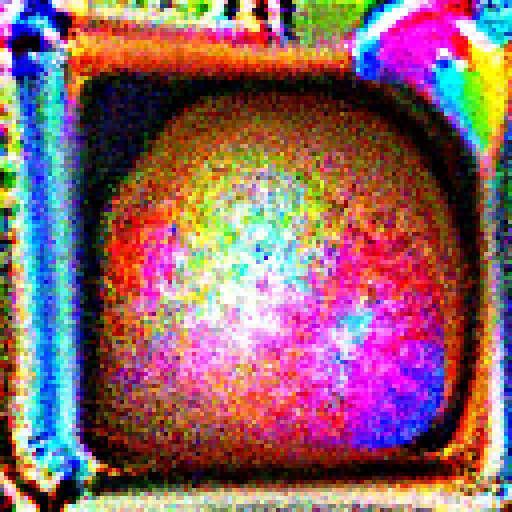
\includegraphics[width=0.155\linewidth]{figures/patch2d_eot.png}\hfill
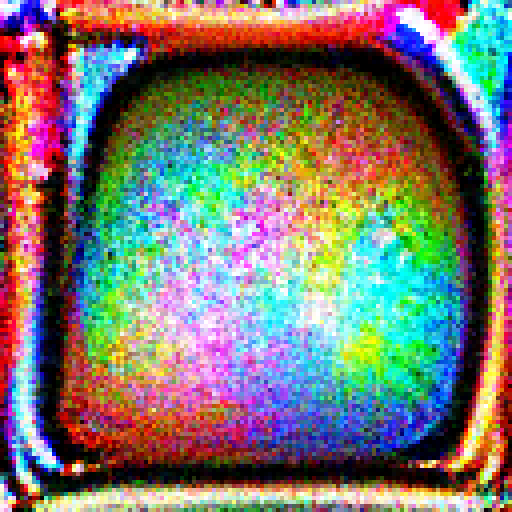
\includegraphics[width=0.155\linewidth]{figures/patch2d_cpa_ls.png}\hfill
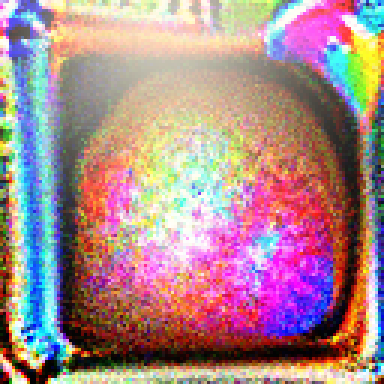
\includegraphics[width=0.155\linewidth]{figures/corr_light.png}\hfill
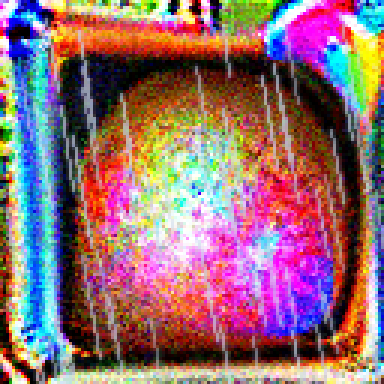
\includegraphics[width=0.155\linewidth]{figures/corr_rain.png}\hfill
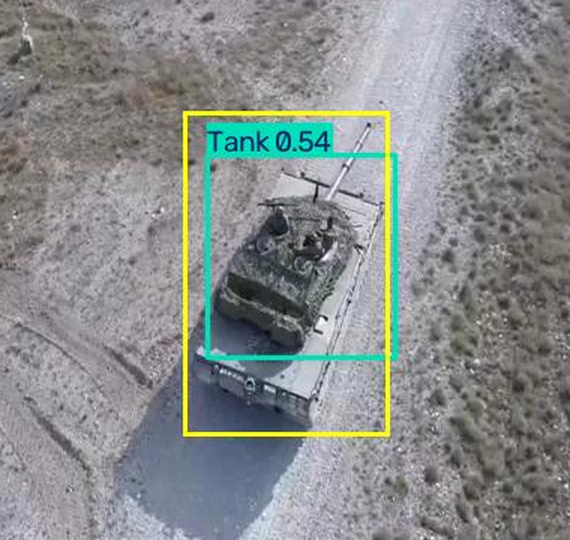
\includegraphics[width=0.155\linewidth]{figures/ex_tank_before.png}\hfill
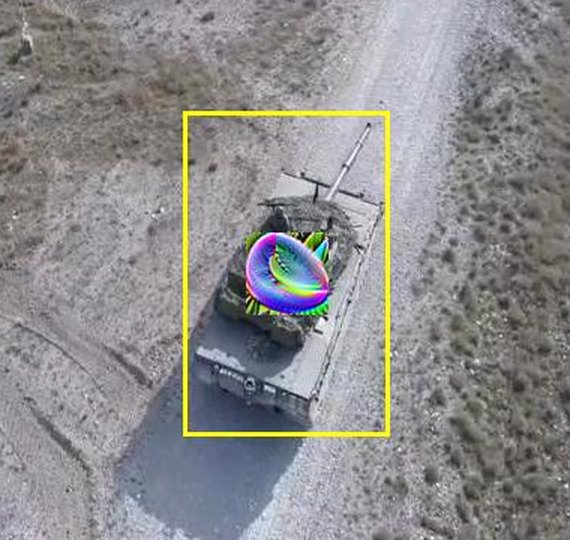
\includegraphics[width=0.155\linewidth]{figures/ex_tank_after.png}
\caption{Stage 1 patches. From left: EOT patch; CPA light+shadow patch; the latter under a light spot and under rain; a held-out tank detected at 0.54 without the patch and not detected with it (YOLOv8s).}
\label{fig:2d}
\end{figure}

\begin{figure}[htbp]
\centering
\begin{subfigure}{0.49\linewidth}\centering
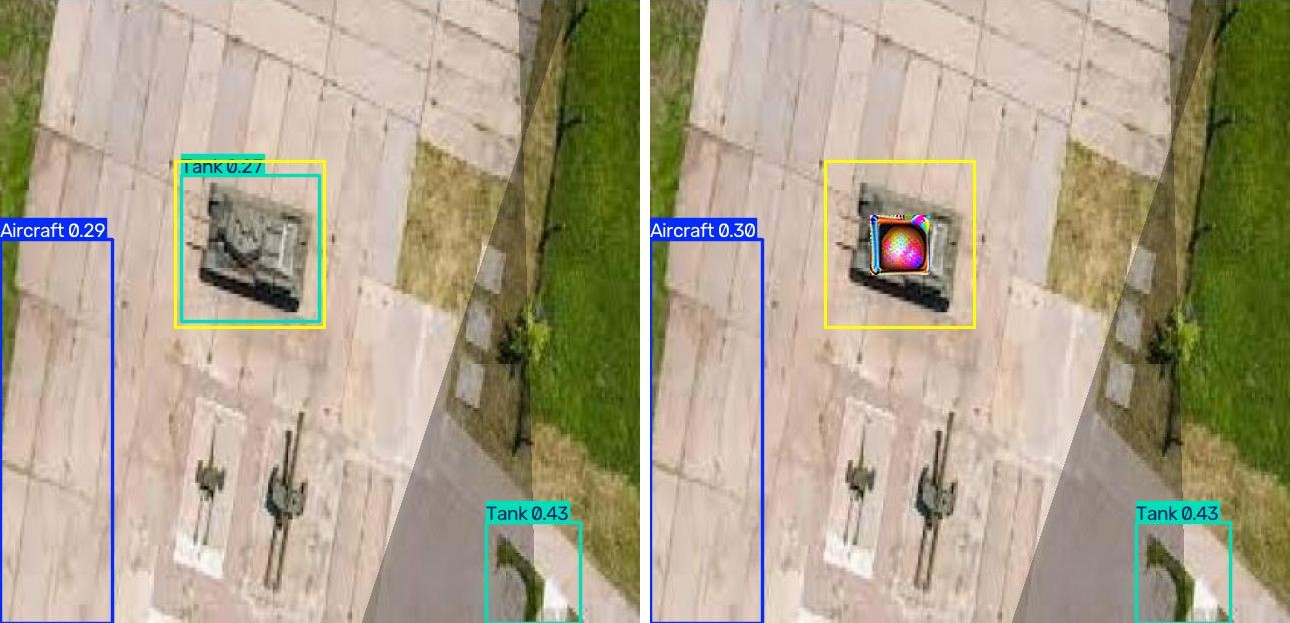
\includegraphics[width=\linewidth]{figures/ex2d_tank_success.jpg}
\caption{Tank, success: 0.27 $\to$ not detected.}
\end{subfigure}\hfill
\begin{subfigure}{0.49\linewidth}\centering
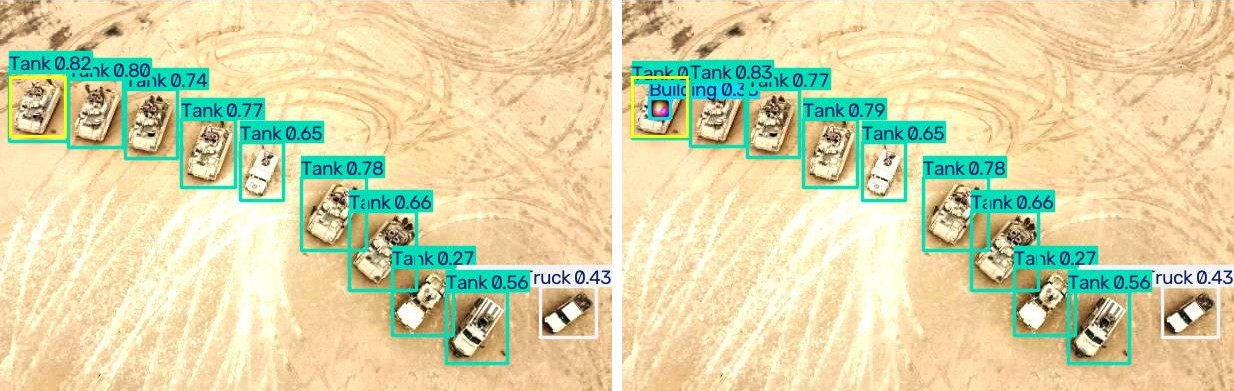
\includegraphics[width=\linewidth]{figures/ex2d_tank_fail.jpg}
\caption{Tank in a convoy, failure: 0.82 $\to$ 0.49.}
\end{subfigure}\\[3pt]
\begin{subfigure}{0.49\linewidth}\centering
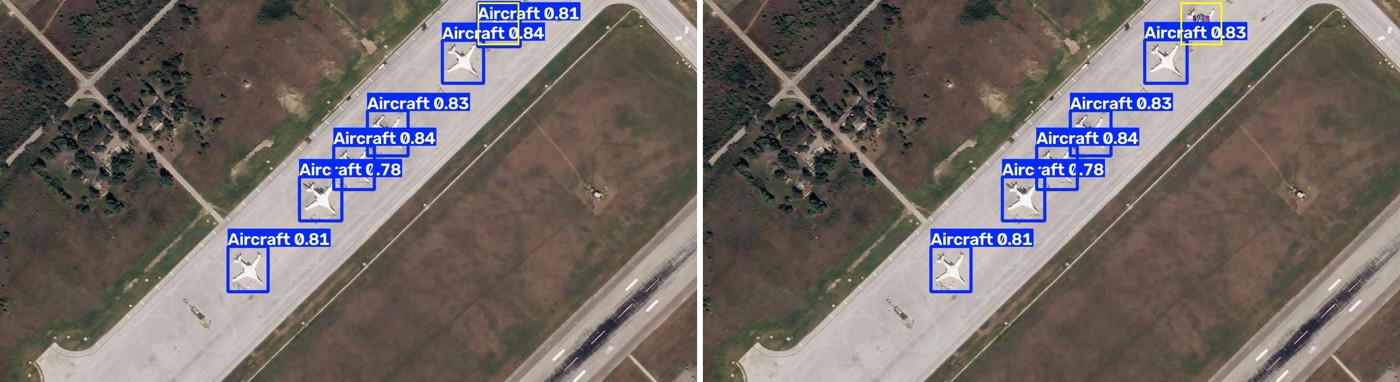
\includegraphics[width=\linewidth]{figures/ex2d_air_success.jpg}
\caption{Aircraft, success.}
\end{subfigure}\hfill
\begin{subfigure}{0.49\linewidth}\centering
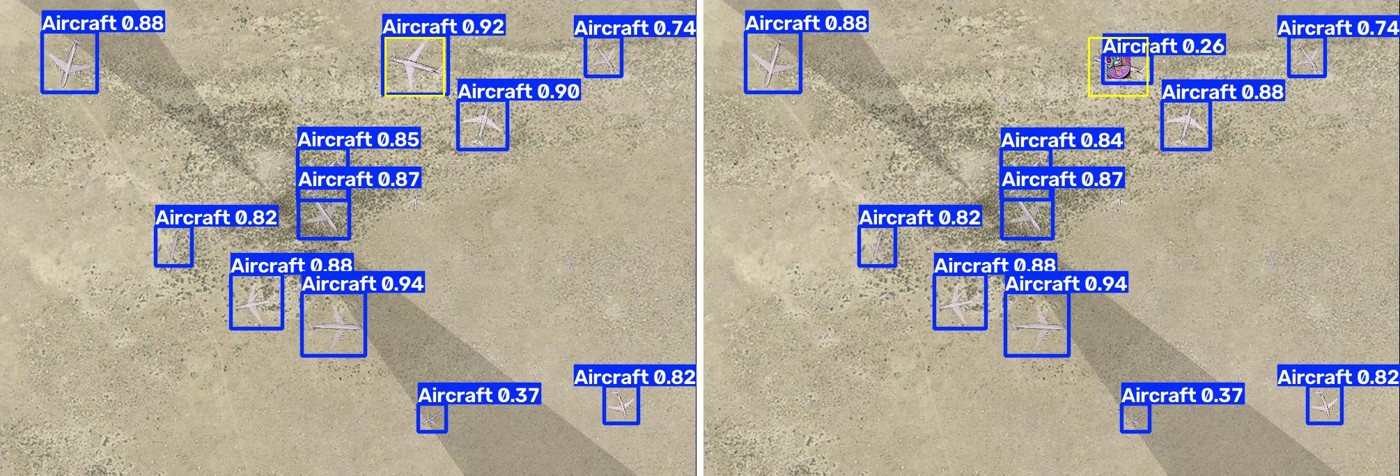
\includegraphics[width=\linewidth]{figures/ex2d_air_fail.jpg}
\caption{Aircraft, failure: 0.92 $\to$ 0.26.}
\end{subfigure}
\caption{Held-out examples of the 2-D EOT patch, before (left half) and after (right half); the attacked instance is boxed in yellow. In both failures the attacked object was detected with high confidence before patching.}
\label{fig:2dex}
\end{figure}

\paragraph{Aircraft.} The same pipeline was run for Aircraft on the DOTA-initialised detector (280 detected aircraft in 21 held-out photographs). Without corruption the patch hides 0.84 of the aircraft, but a gray square of the same relative size already hides 0.78, so the margin is only $+0.06$ \ci{$-0.01$}{$+0.16$} for EOT and $+0.04$ \ci{$-0.05$}{$+0.12$} for CPA light+shadow. Under corruption the margin rises to $+0.14$ \ci{$+0.05$}{$+0.22$} (EOT) and $+0.13$ (CPA), because a gray square loses more of its effect under light and shadow than the pattern does. CPA was again not better than EOT (difference $-0.025$, Holm $p=0.84$). Aircraft are thin, so a square at 0.4 of the box width covers much of the visible fuselage; the class is dominated by occlusion.

\subsection{Effect of the attack on detection metrics across the four classes}\label{sec:res-map}
Table~\ref{tab:mapdrop} reports full-image AP50 on the held-out photographs when the 2-D patch is pasted on every instance of the attacked class, next to the same images with gray and noise squares.

\begin{table}[htbp]
\centering\small
\caption{Full-image AP50 on held-out photographs, mean over 5 folds (3 seeds for Tank, 1 for Aircraft). The patch (0.4 of the box width) is pasted on every instance of the attacked class.}
\label{tab:mapdrop}
\setlength{\tabcolsep}{3.5pt}
\begin{tabular}{@{}llccccc@{}}
\toprule
Attacked class & Images & Aircraft & Building & Mil.\ Truck & Tank & mAP50 \\
\midrule
\multirow{7}{*}{Tank (YOLOv8s)} & clean & 0.310 & 0.239 & 0.052 & 0.156 & 0.189 \\
 & gray square & 0.316 & 0.227 & 0.053 & 0.052 & 0.162 \\
 & noise square & 0.316 & 0.232 & 0.053 & 0.067 & 0.167 \\
 & EOT patch & 0.297 & 0.226 & 0.054 & \textbf{0.019} & 0.149 \\
 & CPA light patch & 0.299 & 0.220 & 0.054 & \textbf{0.018} & 0.148 \\
 & CPA shadow patch & 0.302 & 0.216 & 0.055 & \textbf{0.013} & 0.147 \\
 & CPA light+shadow patch & 0.306 & 0.215 & 0.055 & \textbf{0.009} & 0.146 \\
\midrule
\multirow{5}{*}{\shortstack[l]{Aircraft (YOLOv8s,\\ DOTA init.)}} & clean & 0.431 & 0.337 & 0.093 & 0.190 & 0.263 \\
 & gray square & 0.053 & 0.337 & 0.091 & 0.188 & 0.167 \\
 & noise square & 0.092 & 0.332 & 0.092 & 0.189 & 0.176 \\
 & EOT patch & \textbf{0.009} & 0.320 & 0.088 & 0.153 & 0.143 \\
 & CPA light+shadow patch & \textbf{0.010} & 0.318 & 0.089 & 0.158 & 0.144 \\
\bottomrule
\end{tabular}
\end{table}

The attack is class-specific: the attacked class collapses while the other classes change by at most 0.04, so mAP50 falls (0.189 $\to$ 0.146) almost entirely through the attacked class. For Tank, the patch removes 88--94\,\% of the clean AP50 (0.156 $\to$ 0.009--0.019), whereas a gray square of the same size removes 67\,\%; the adversarial pattern is responsible for the difference. For Aircraft, occlusion alone removes 88\,\% of the AP50 and the pattern adds little (0.053 $\to$ 0.009). Military Truck (AP50 0.05) is not detected well enough to be attacked, and Building is a static structure for which a patch has no comparable physical meaning; neither was targeted.

The 2-D stage established that a pattern beats occlusion on unseen photographs, but at a size that cannot be printed and placed reliably (Section~\ref{sec:2d}). Stage 2 keeps the evaluation and makes the attack physical.

\subsection{Stage 2: the printable 3-D patch}\label{sec:res-3d}
Table~\ref{tab:3d} gives the attack success and margin of the four 3-D CPA textures (trained on YOLOv8s) on all four detectors. The 1\,m sheet hides 0.31--0.50 of the detected tanks and \textbf{12--27 points more than a gray or noise sheet of the same size on every detector}, including the three black-box detectors; for \emph{none} and \emph{light+shadow} all black-box intervals exclude zero. Figure~\ref{fig:examples} shows two held-out tanks that disappear once the sheet is on the roof, and the patches compared in this report.

\begin{table}[htbp]
\centering\small
\caption{3-D CPA, 1\,m sheet, trained on YOLOv8s, confidence 0.5. ASR and margin over the best same-size control [95\,\% photo-level interval]. $n$: tanks detected before patching.}
\label{tab:3d}
\setlength{\tabcolsep}{2.5pt}\footnotesize
\begin{tabular}{@{}lcccc@{}}
\toprule
 & YOLOv8s (white-box) & YOLOv8m & YOLO11s & RT-DETR-l \\
 & $n=143$, 13 photos & $n=178$, 16 photos & $n=135$, 14 photos & $n=158$, 17 photos \\
\midrule
\multicolumn{5}{@{}l}{\textit{ASR}}\\
none & 0.315 & 0.348 & 0.496 & 0.443 \\
light+shadow & 0.315 & 0.326 & 0.504 & 0.418 \\
gray / noise sheet & 0.161 / 0.112 & 0.213 / 0.152 & 0.378 / 0.244 & 0.177 / 0.158 \\
\midrule
\multicolumn{5}{@{}l}{\textit{Margin over best control}}\\
none & $+0.154$ \ci{$+0.00$}{$+0.38$} & $+0.135$ \ci{$+0.07$}{$+0.20$} & $+0.119$ \ci{$+0.02$}{$+0.24$} & $+0.266$ \ci{$+0.14$}{$+0.43$} \\
light & $+0.126$ \ci{$-0.01$}{$+0.35$} & $+0.174$ \ci{$+0.09$}{$+0.24$} & $+0.111$ \ci{$-0.01$}{$+0.27$} & $+0.247$ \ci{$+0.12$}{$+0.39$} \\
shadow & $+0.140$ \ci{$-0.01$}{$+0.37$} & $+0.135$ \ci{$+0.06$}{$+0.23$} & $+0.096$ \ci{$-0.02$}{$+0.23$} & $+0.215$ \ci{$+0.11$}{$+0.33$} \\
light+shadow & $+0.154$ \ci{$+0.03$}{$+0.35$} & $+0.112$ \ci{$+0.04$}{$+0.18$} & $+0.126$ \ci{$+0.02$}{$+0.26$} & $+0.241$ \ci{$+0.13$}{$+0.38$} \\
\bottomrule
\end{tabular}
\end{table}

\begin{figure}[htbp]
\centering
\begin{subfigure}{\linewidth}\centering
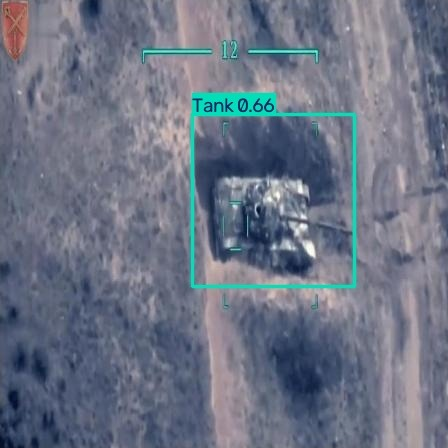
\includegraphics[width=0.235\linewidth]{figures/ex1_before.jpg}\hfill
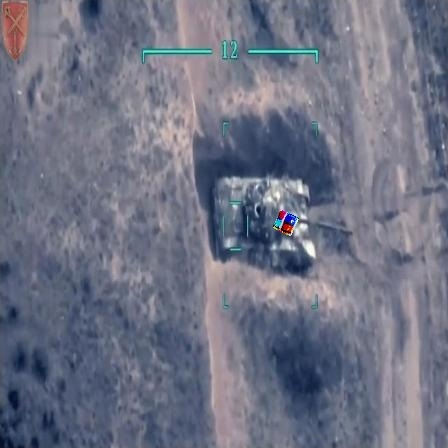
\includegraphics[width=0.235\linewidth]{figures/ex1_after.jpg}\hfill
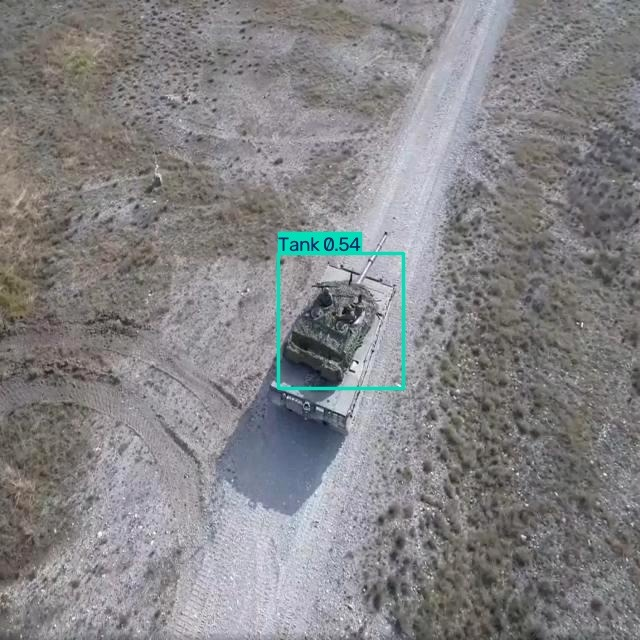
\includegraphics[width=0.235\linewidth]{figures/ex2_before.jpg}\hfill
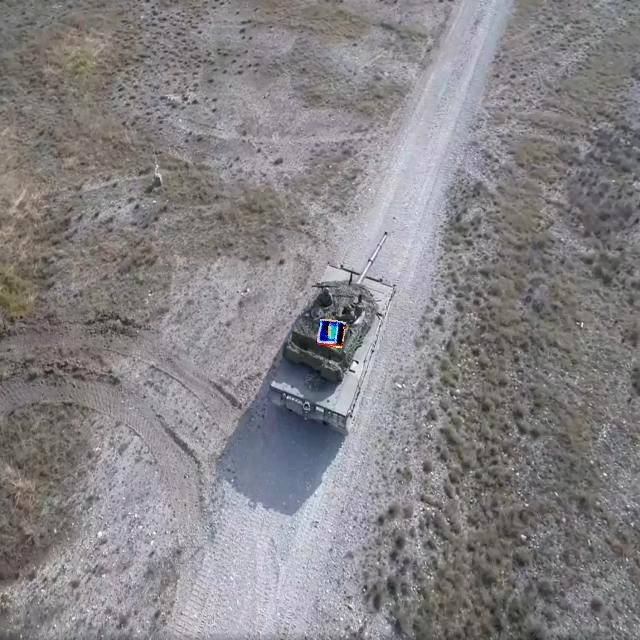
\includegraphics[width=0.235\linewidth]{figures/ex2_after.jpg}
\caption{Held-out photographs, YOLOv8s at confidence 0.5: Tank 0.66 $\to$ not detected; Tank 0.54 $\to$ not detected (3-D CPA, \emph{none}).}
\end{subfigure}\\[4pt]
\begin{subfigure}{\linewidth}\centering
\setlength{\tabcolsep}{2pt}
\begin{tabular}{cccccc}
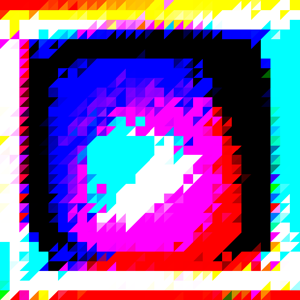
\includegraphics[width=0.145\linewidth]{figures/patch_cpa_none.png} &
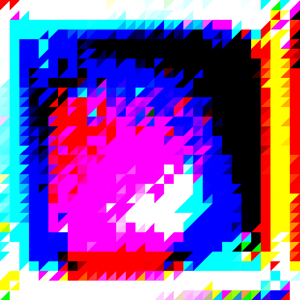
\includegraphics[width=0.145\linewidth]{figures/patch_cpa_ls.png} &
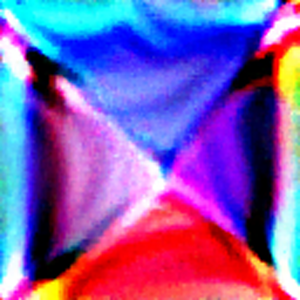
\includegraphics[width=0.145\linewidth]{figures/patch_pixel.png} &
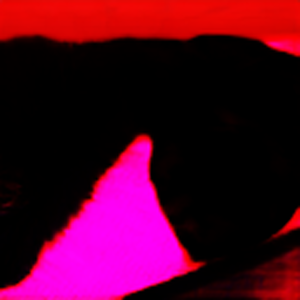
\includegraphics[width=0.145\linewidth]{figures/patch_npa_dog.png} &
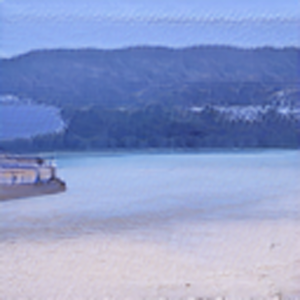
\includegraphics[width=0.145\linewidth]{figures/patch_npa_stop.png} &
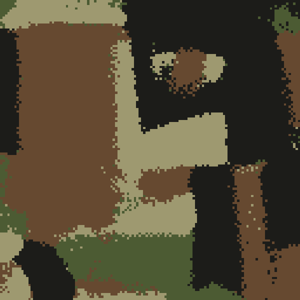
\includegraphics[width=0.145\linewidth]{figures/patch_camo.png} \\
\footnotesize CPA none & \footnotesize CPA light+shadow & \footnotesize pixel (no GAN) & \footnotesize NPA, $\tau=10$ & \footnotesize NPA, early stop & \footnotesize camouflage \\
\footnotesize $+0.17$ & \footnotesize $+0.16$ & \footnotesize $+0.17$ & \footnotesize $+0.18$ & \footnotesize $+0.10$ & \footnotesize $+0.01$ \\
\end{tabular}
\caption{Printable 1\,m patches (fold 1) with their margin over the best control, mean of the 4 detectors.}
\end{subfigure}
\caption{The 3-D attacks on held-out photographs and the patches compared in this report.}
\label{fig:examples}
\end{figure}

\paragraph{Robustness to conditions.} Figure~\ref{fig:robust} shows the margin of the \emph{none} texture under each test condition. The pattern keeps a positive margin under light spots and shadows and under rain and mud, which it never saw. Raw ASR \emph{increases} under rain and mud (for example 0.44 $\to$ 0.61 on RT-DETR), but it increases equally for the gray sheet (0.18 $\to$ 0.47): most of the apparent gain under bad weather is the weather hiding the vehicle, not the patch. Shadows reduce the margin most on the YOLOv8 detectors, because a shadowed gray sheet already hides many tanks.

\begin{figure}[htbp]
\centering
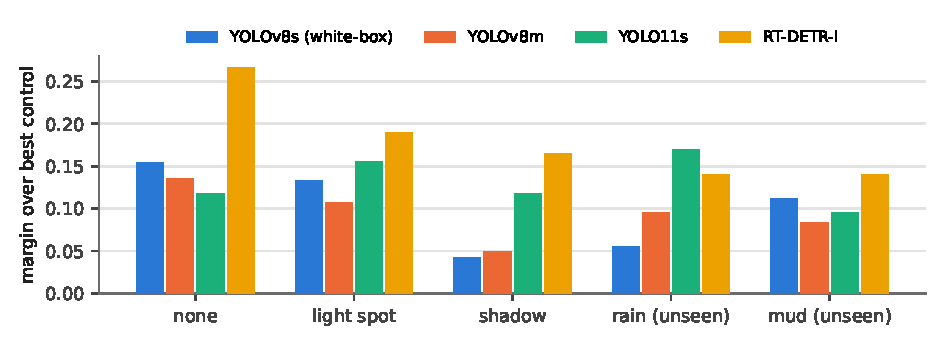
\includegraphics[width=0.9\linewidth]{figures/robustness.pdf}
\caption{Margin of the 3-D \emph{none} texture over the best same-size control under each test condition (confidence 0.5). Rain and mud were not used in training.}
\label{fig:robust}
\end{figure}

\paragraph{Training behaviour.} Figure~\ref{fig:train}a shows the share of training tanks scored below 0.5 during 3-D CPA training, averaged over the folds. It rises from 0.62--0.67 to 0.76--0.79 within ten epochs, with most of the gain in the first two epochs, which supports the paper's 10-epoch schedule. The corruption-trained variants end slightly higher on their training images, because the light spot and the shadow themselves lower the score of some tanks; this training-time advantage does not carry over to clean test images (Table~\ref{tab:3d}).

\begin{figure}[htbp]
\centering
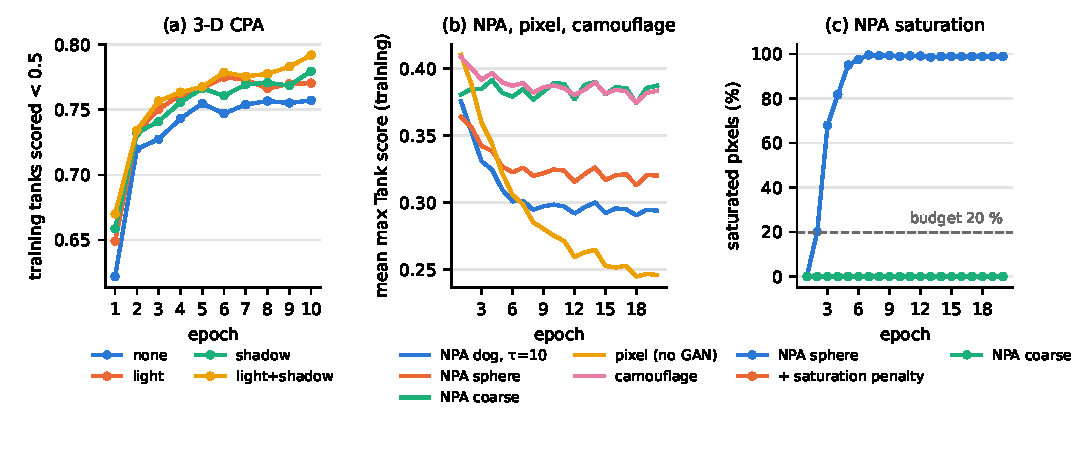
\includegraphics[width=\linewidth]{figures/training_curves.pdf}
\caption{Training curves, mean over folds. (a) 3-D CPA: share of training tanks with per-tank score below 0.5. (b) NPA, pixel and camouflage: mean per-tank maximum Tank score. (c) Saturated pixels of the NPA patch per epoch (the early-stop variant keeps the last epoch below the 20\,\% line).}
\label{fig:train}
\end{figure}

\paragraph{Lower confidence threshold.} At confidence 0.25 the sample grows to 185--244 detected tanks per detector and the conclusions are unchanged: margins of $+0.07$ to $+0.24$ on all detectors (Table~\ref{tab:a-025}). Light+shadow is 0.02--0.03 above \emph{none} on three detectors at this threshold, but the paired black-box comparison remains null ($+0.002$ \ci{$-0.01$}{$+0.02$}, Section~\ref{sec:res-transfer}). Per-condition ASR for every texture and control is in Table~\ref{tab:a-cond}.

\paragraph{The CPA ablation.} The four textures perform alike: every light, shadow or light+shadow minus none difference is at most 0.05 in magnitude, and none of the 24 paired tests (3 variants $\times$ 2 conditions $\times$ 4 detectors) is significant after Holm correction (largest difference: shadow on RT-DETR, $-0.051$, adjusted $p=0.94$). The improvement reported by the paper (15.5\,\% $\to$ 20.8\,\% with light and shadow) does not appear.

\subsection{Transferability}\label{sec:res-transfer}
Figure~\ref{fig:transfer} shows the transfer matrices, Table~\ref{tab:transfer} their summary, and Table~\ref{tab:a-transfer} every cell with its interval.

\begin{figure}[htbp]
\centering
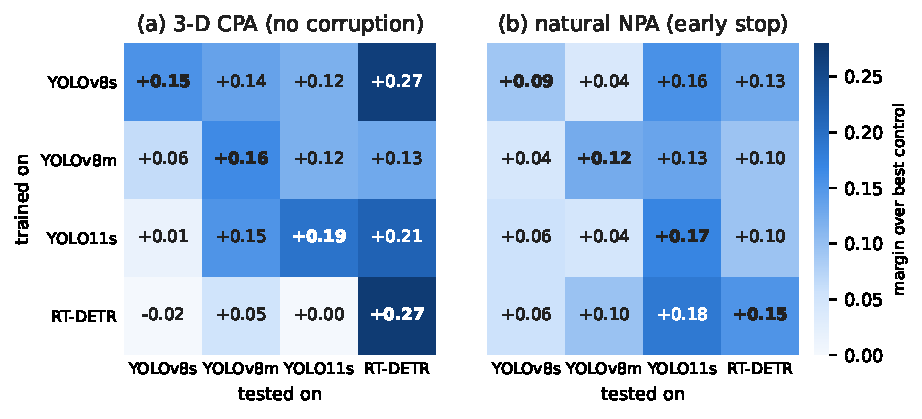
\includegraphics[width=0.92\linewidth]{figures/transfer.pdf}
\caption{Transfer matrices (margin over the best control, confidence 0.5). Rows: detector used for training; columns: detector tested. Diagonal (bold): white-box.}
\label{fig:transfer}
\end{figure}

\begin{table}[htbp]
\centering\small
\caption{Transfer summary: mean margin on the 4 white-box and 12 black-box cells, and paired comparisons over all black-box pairs.}
\label{tab:transfer}
\begin{tabular}{@{}lccc@{}}
\toprule
Attack & white-box $W$ & black-box $B$ & $B/W$ \\
\midrule
3-D CPA, none & $+0.195$ & $+0.103$ & 0.53 \\
3-D CPA, light+shadow & $+0.196$ & $+0.099$ & 0.51 \\
NPA, early stop & $+0.134$ & $+0.094$ & 0.70 \\
\midrule
\multicolumn{4}{@{}l}{\textit{Paired tests, pooled over the 12 black-box pairs}} \\
CPA claim: light+shadow $-$ none & \multicolumn{3}{l}{$-0.004$ \ci{$-0.02$}{$+0.01$}, $p=0.73$} \\
NPA early stop $-$ CPA none & \multicolumn{3}{l}{$-0.015$ \ci{$-0.05$}{$+0.02$}, $p=0.54$} \\
\quad tested on RT-DETR only & \multicolumn{3}{l}{$-0.097$ \ci{$-0.15$}{$-0.05$}, Holm $p=0.007$} \\
\bottomrule
\end{tabular}
\end{table}

\begin{itemize}
  \item \textbf{Patches transfer}: about half of the white-box margin survives on detectors the attacker never used.
  \item \textbf{Transfer is asymmetric}: patches trained on the convolutional YOLO detectors transfer strongly to the transformer RT-DETR ($+0.13$ to $+0.27$), but the CPA patch trained on RT-DETR does not reach the YOLO detectors ($-0.02$ to $+0.05$). The natural NPA patch trained on RT-DETR does ($+0.06$ to $+0.19$), and NPA keeps 70\,\% of its white-box effect versus 51--53\,\% for CPA, consistent with the GAN removing surrogate-specific high-frequency structure.
  \item \textbf{Corruption training does not improve transfer}: pooled over all black-box pairs the difference is $-0.004$ with interval $[-0.02,+0.01]$, which excludes the paper's $+0.05$; at confidence 0.25 it is $+0.002$ \ci{$-0.01$}{$+0.02$}.
\end{itemize}

\subsection{Why does corruption training not help?}\label{sec:res-why}
Four ablations test explanations (Table~\ref{tab:ablation}; gains are light+shadow minus none on the black-box detectors).

\begin{table}[htbp]
\centering\small
\caption{CPA gain (light+shadow $-$ none) on black-box detectors under four ablations, confidence 0.5.}
\label{tab:ablation}
\begin{tabularx}{\linewidth}{@{}p{5.4cm}Yp{3.7cm}@{}}
\toprule
Ablation & Question & Gain \\
\midrule
Sheet 1 / 1.5 / 2\,m & Does a gain appear for stronger patches? & $-0.03$ to $+0.15$, none Holm-significant \\
Two seeds, averaged & Does averaging reveal a small gain? & $-0.02$ to $+0.02$ \\
Corruption probability 1.0 & Does more corruption help? & $-0.02$ to $+0.02$ \\
Paper-like fixed view per tank (2 seeds) & Is our view diversity masking the gain? & $-0.005$ \ci{$-0.02$}{$+0.01$} \\
\quad interaction (low $-$ full diversity) & & $-0.008$ \ci{$-0.03$}{$+0.02$}, $p=0.63$ \\
\midrule
\textit{Seed-to-seed change, same method} & & \textit{up to} $\pm0.06$ \\
\textit{Gain reported by the paper} & & $+0.053$ \textit{(single run)} \\
\bottomrule
\end{tabularx}
\end{table}

\paragraph{Patch size.} Larger sheets raise the raw ASR mostly through occlusion: at 2\,m a gray or noise sheet alone hides 40--72\,\% of the tanks, and on YOLO11s the 2\,m adversarial margin is even negative ($-0.095$). No size produces a consistent gain; the one large value ($+0.15$, YOLOv8m at 1.5\,m) has adjusted $p=0.23$ (full results in Table~\ref{tab:a-size}).

\paragraph{Seeds and corruption strength.} Retraining the same method with another seed changes its margin by up to 0.06 on a detector, the size of the gain the paper reports from a single run. Averaging two seeds or corrupting every image produces no gain (Tables~\ref{tab:a-seed} and~\ref{tab:a-p}).

\paragraph{Training diversity.} The most plausible explanation was that the paper's baseline sees each car from one simulator pose, so corruptions are its main source of variation, while ours already varies view, lighting and heading every step. Training with one fixed view and heading per tank (the paper's regime) gives the same null gain, and the interaction is $-0.008$ ($p=0.63$), so this explanation is rejected (per-detector results in Table~\ref{tab:a-div}).

\paragraph{Inference.} The implementation follows the authors' code, and the corruptions were verified to be active during training. On real aerial photographs and four modern detectors, pattern corruption does not improve transferability; the published evidence is a single run per configuration, with a gain comparable to run-to-run variation.

\subsection{Stage 3: naturalistic patches}\label{sec:res-npa}
Table~\ref{tab:npa} reports attack margin and naturalness of all GAN, pixel and camouflage patches, Figure~\ref{fig:gallery} shows them, and Tables~\ref{tab:a-npa} and~\ref{tab:a-nat} give the per-detector margins and all naturalness proxies.

\begin{table}[htbp]
\centering\small
\caption{Naturalistic patches: margin over the best control (mean of the 4 detectors, confidence 0.5) and saturated pixels (mean over folds).}
\label{tab:npa}
\begin{tabular}{@{}llcc@{}}
\toprule
Group & Patch & margin & saturated \\
\midrule
\multirow{4}{*}{NPA as in the paper} & dog (259), $\tau=10$ & $+0.183$ & 98.9\,\% \\
 & dog, $\tau=4$ & $+0.171$ & 98.4\,\% \\
 & dog, $\tau=2$ & $+0.133$ & 97.2\,\% \\
 & dog, start image (not optimised) & $+0.003$ & 0.9\,\% \\
\midrule
\multirow{2}{*}{Scene classes, $\tau=4$} & hay (958) & $+0.151$ & 100\,\% \\
 & sandbar (977) & $+0.223$ & 100\,\% \\
\midrule
\multirow{4}{*}{Remedies (977, $\tau=3$)} & latent on sphere & $+0.198$ & 87.5\,\% \\
 & + coarse latent only & $+0.050$ & 0.0\,\% \\
 & + saturation penalty & $+0.163$ & 0.0\,\%$^\ast$ \\
 & \textbf{+ early stop, $S=20\,\%$} & $\mathbf{+0.103}$ & \textbf{7.8\,\%} \\
\midrule
Baselines & pixel patch (no GAN) & $+0.173$ & 64.8\,\% \\
 & 3-D CPA, none & $+0.169$ & -- \\
\midrule
\multirow{3}{*}{Camouflage (AdvCaT)} & woodland, 1\,m & $+0.013$ & 0\,\% \\
 & tank colours, 1\,m & $-0.007$ & 0\,\% \\
 & woodland, 3\,m & $-0.031$ & 0\,\% \\
\bottomrule
\multicolumn{4}{@{}l}{\footnotesize $^\ast$passes the metric but is visibly unnatural (Figure~\ref{fig:gallery}).}
\end{tabular}
\end{table}

\begin{figure}[htbp]
\centering
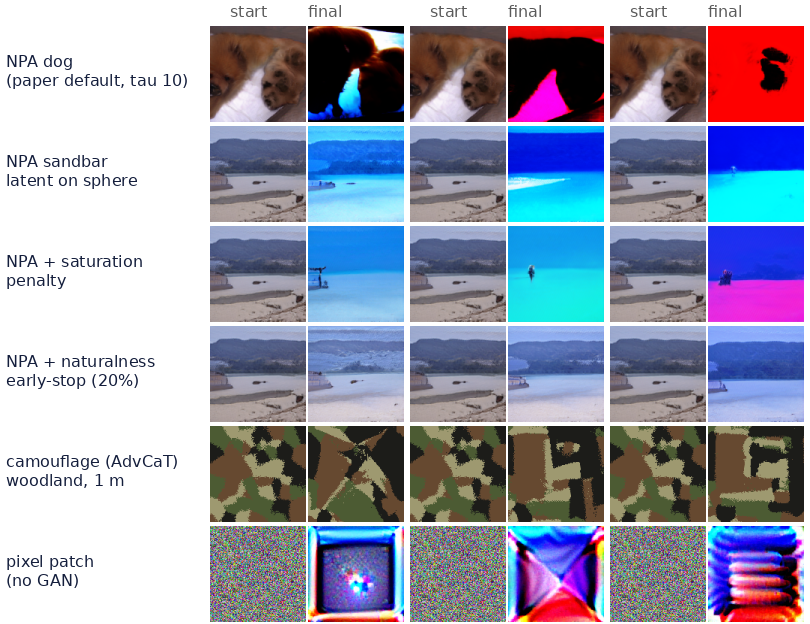
\includegraphics[width=0.78\linewidth]{figures/patch_gallery.png}
\caption{Start and final patch for three folds of each method. Only the early-stopped NPA keeps a recognisable scene while attacking.}
\label{fig:gallery}
\end{figure}

\paragraph{The latent clamp does not control realism.} With the paper's settings the dog image becomes saturated colour blocks within a few epochs (98.9\,\% saturated). Tightening the clamp to $\tau=2$ lowers the attack ($+0.18\to+0.13$) but not the saturation (97.2\,\%). At $\tau=10$ the largest final latent component was only 4.3, so the clamp never acted; at $\tau=2$ it acted on every component and the image still saturated. As derived in Section~\ref{sec:npa}, a box bound limits each component separately: with all 120 components near $\pm2$ the norm is $\approx22$, twice the typical $\sqrt{120}\approx11$, far outside what the generator was trained on. The start image has a margin of zero, so the NPA effect comes from the optimisation and not from placing a picture on the vehicle.

\paragraph{Optimisation behaviour.} Figure~\ref{fig:train}b explains the ranking. The pixel patch, with the most freedom, lowers the training score most (0.41 $\to$ 0.25); the unconstrained GAN latent follows (dog: 0.38 $\to$ 0.29; sphere: 0.36 $\to$ 0.32). The coarse latent and the camouflage patterns barely move the score (0.38--0.41 throughout), which is why their test margins are close to zero: their parameterisations cannot express an adversarial pattern. Figure~\ref{fig:train}c shows how fast naturalness is lost on the sphere: about 20\,\% of the pixels are saturated after two epochs, 68\,\% after three and over 95\,\% after five, while the saturation penalty and the coarse latent stay at 0\,\%.

\paragraph{Remedies.} Keeping $z$ on the typical shell kept a strong attack ($+0.20$) but still left 88\,\% of the pixels saturated, because directions on the shell can also produce extreme images. Optimising only the coarse latent stayed natural but lost the attack ($+0.05$). The saturation penalty drove the metric to zero, but the result is visibly artificial (flat posterised blocks): once a statistic is optimised directly it stops measuring naturalness. The naturalness-budget early stop kept a recognisable scene with 7.8\,\% saturation and a margin of $+0.10$.

\paragraph{Realism--attack trade-off.} Figure~\ref{fig:tradeoff} varies the budget along the same training runs. The trade-off is smooth and monotone: the start image (0\,\% saturated) has no effect, one epoch (1.2\,\%) already gives $+0.07$, the 20\,\% budget $+0.10$, and the unconstrained final patch (99\,\%) $+0.22$. More than half of the pixels saturate within 2--4 of the 20 epochs. A photo-like patch therefore retains about half of the attack of an unconstrained one and, as shown in Section~\ref{sec:res-transfer}, transfers as well as CPA on average.

\begin{figure}[htbp]
\centering
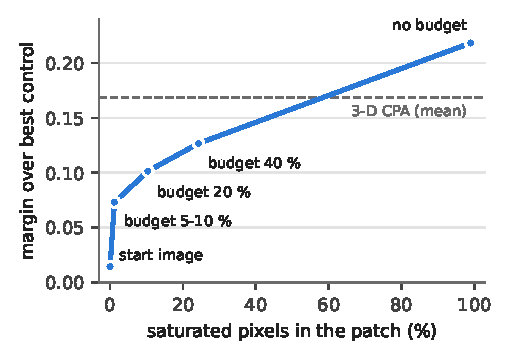
\includegraphics[width=0.5\linewidth]{figures/tradeoff.pdf}
\caption{Realism--attack trade-off of NPA: each point is the epoch selected by a saturation budget on the same five training runs (mean margin over 4 detectors).}
\label{fig:tradeoff}
\end{figure}

\paragraph{Camouflage.} AdvCaT patterns are natural by construction but do not beat a gray sheet (margins $-0.01$ to $+0.01$ at 1\,m, negative at 3\,m, where a gray sheet already hides 71--88\,\% of the tanks). Optimisation helps relative to a random camouflage of the same palette ($+0.04$ to $+0.12$ for woodland), but random camouflage starts \emph{below} the gray control ($-0.06$ on average), plausibly because it resembles vehicle paint while a gray sheet breaks up the vehicle's appearance. With four colours and movable region boundaries the pattern has too few degrees of freedom to carry an attack. Note also that ``natural'' in NPA means photo-like rather than appropriate to the context: a coastal scene on a tank roof passes a pixel statistic but would be noticed by an analyst, and the only context-appropriate option, camouflage, did not attack.

\subsection{Discussion}\label{sec:discussion}
\paragraph{Answers to the questions of Section~\ref{sec:intro}.}
\begin{enumerate}
  \item The patch removes nearly all Tank detections from the full-image metric (AP50 $0.156\to0.009$) and the printable 1\,m sheet hides 12--27 points more tanks than occlusion; the effect is specific to the attacked class.
  \item CPA does not improve robustness or transfer beyond the EOT/none baseline in any of the tests.
  \item NPA can be natural and adversarial only with an explicit naturalness budget; the latent clamp alone is not enough, and a natural patch keeps about half the attack.
  \item About half of the effect transfers to unseen detectors, strongly from CNNs to the transformer and weakly in the reverse direction, so a black-box attacker without the defender's weights remains effective.
  \item Light spots and shadows reduce the margin modestly, rain and mud hide vehicles on their own, and larger sheets work mostly through occlusion.
\end{enumerate}

\paragraph{Effect of the evaluation design.} The protocol changed conclusions in three places. A file-level split would have reported mAP50 $=0.86$ instead of 0.20. Without occlusion controls, larger patches and bad weather would have appeared to strengthen the attack. Without photo-level statistics and repeated seeds, differences of 0.05, the size of the CPA claim, would have looked meaningful, while seed-to-seed variation alone reaches 0.06.

\paragraph{Threats to validity.} All attacks are digital: rendered onto real photographs, not printed and flown. Only the sheet is rendered from sampled viewpoints while the photograph keeps its own, and the roof mesh is procedural. The dataset has 88 photographs, and only 13--17 held-out photographs contain tanks that each detector finds, so intervals are wide; conclusions rest on effects consistent across detectors and ablations, or on intervals that exclude the claimed effect. Naturalness was judged by a proxy and by eye, not by a user study.

%=====================================================================
\section{Conclusions}\label{sec:conclusion}
\begin{enumerate}
  \item A fine-tuned YOLOv8s reaches mAP50 0.20 on unseen photographs and 0.44 on the official test split; Tank and Aircraft are detected, Military Truck almost never.
  \item An adversarial patch collapses the attacked class (Tank AP50 $0.156\to0.009$) without affecting the others; for a printable 1\,m 3-D sheet guaranteed to lie on the vehicle, the pattern hides 12--27 points more tanks than a gray sheet on one white-box and three black-box detectors.
  \item About half of the white-box effect transfers to unseen detectors; transfer from convolutional detectors to RT-DETR is strong, the reverse weak.
  \item The added structure of CPA gives no measurable benefit: the pooled black-box gain of corruption training is $-0.004$ \ci{$-0.02$}{$+0.01$}, and it stays null for larger patches, averaged seeds, stronger corruption and the paper's low-diversity regime.
  \item NPA's latent clamp does not keep patches natural; a naturalness-budget early stop yields photo-like patches that keep about half the attack and retain 70\,\% of it on unseen detectors. Four-colour camouflage is too constrained to attack.
  \item Occlusion controls, photo-grouped splits, photo-level statistics and repeated seeds are necessary to draw these conclusions from a small aerial dataset.
\end{enumerate}

\paragraph{Limitations and future work.} The next steps are a physical test (a printed sheet on a scale model photographed by a drone), a human naturalness survey, re-running the CPA authors' code on their simulator data with several seeds, context-appropriate natural priors (terrain-trained or diffusion generators, style losses towards vehicle paint), a stratified analysis by object size, and defences such as patch detection and input purification.

\section*{Code availability}
All code, the result tables and the source of this report are available at \url{\repo}. The repository contains dataset preparation, photo-grouped cross-validation, detector training and evaluation, the 2-D patch attacks, the 3-D CPA, NPA and camouflage attacks, and the analysis scripts that produce every table. The dataset is not included because of the course instructor's restriction.

%=====================================================================
\begin{thebibliography}{99}\small
\setlength{\itemsep}{1pt}
\bibitem{szegedy2014} C.~Szegedy, W.~Zaremba, I.~Sutskever, J.~Bruna, D.~Erhan, I.~Goodfellow, R.~Fergus. Intriguing properties of neural networks. \emph{ICLR}, 2014.
\bibitem{goodfellow2015} I.~J.~Goodfellow, J.~Shlens, C.~Szegedy. Explaining and harnessing adversarial examples. \emph{ICLR}, 2015.
\bibitem{kurakin2017} A.~Kurakin, I.~Goodfellow, S.~Bengio. Adversarial examples in the physical world. \emph{ICLR Workshop}, 2017. arXiv:1607.02533.
\bibitem{sharif2016} M.~Sharif, S.~Bhagavatula, L.~Bauer, M.~K.~Reiter. Accessorize to a crime: real and stealthy attacks on state-of-the-art face recognition. \emph{ACM CCS}, 2016.
\bibitem{eykholt2018} K.~Eykholt, I.~Evtimov, E.~Fernandes, B.~Li, A.~Rahmati, C.~Xiao, A.~Prakash, T.~Kohno, D.~Song. Robust physical-world attacks on deep learning visual classification. \emph{CVPR}, 2018.
\bibitem{athalye2018} A.~Athalye, L.~Engstrom, A.~Ilyas, K.~Kwok. Synthesizing robust adversarial examples. \emph{ICML}, 2018.
\bibitem{brown2017} T.~B.~Brown, D.~Man\'e, A.~Roy, M.~Abadi, J.~Gilmer. Adversarial patch. arXiv:1712.09665, 2017.
\bibitem{chen2018shapeshifter} S.-T.~Chen, C.~Cornelius, J.~Martin, D.~H.~Chau. ShapeShifter: robust physical adversarial attack on Faster R-CNN object detector. \emph{ECML-PKDD}, 2018.
\bibitem{thys2019} S.~Thys, W.~Van~Ranst, T.~Goedem\'e. Fooling automated surveillance cameras: adversarial patches to attack person detection. \emph{CVPR Workshops}, 2019.
\bibitem{xu2020tshirt} K.~Xu et al. Adversarial T-shirt! Evading person detectors in a physical world. \emph{ECCV}, 2020.
\bibitem{wu2020cloak} Z.~Wu, S.-N.~Lim, L.~S.~Davis, T.~Goldstein. Making an invisibility cloak: real world adversarial attacks on object detectors. \emph{ECCV}, 2020.
\bibitem{huang2020upc} L.~Huang et al. Universal physical camouflage attacks on object detectors. \emph{CVPR}, 2020.
\bibitem{wang2021das} J.~Wang et al. Dual attention suppression attack: generate adversarial camouflage in physical world. \emph{CVPR}, 2021.
\bibitem{wang2022fca} D.~Wang et al. FCA: learning a 3D full-coverage vehicle camouflage for multi-view physical adversarial attack. \emph{AAAI}, 2022.
\bibitem{suryanto2022dta} N.~Suryanto et al. DTA: physical camouflage attacks using differentiable transformation network. \emph{CVPR}, 2022.
\bibitem{denhollander2020} R.~den~Hollander et al. Adversarial patch camouflage against aerial detection. \emph{Proc.\ SPIE} 11543, 2020.
\bibitem{du2022aerial} A.~Du et al. Physical adversarial attacks on an aerial imagery object detector. \emph{WACV}, 2022.
\bibitem{tang2024de} G.~Tang et al. Black-box adversarial patch attacks using differential evolution against aerial imagery object detectors. \emph{Engineering Applications of Artificial Intelligence}, 2024.
\bibitem{zhang2024cpa} Y.~Zhang, Z.~Gong, H.~Wen, X.~Hu, X.~Xia, H.~Jiang, P.~Zhong. Pattern corruption-assisted physical attacks against object detection in UAV remote sensing. \emph{IEEE J.\ Sel.\ Topics Appl.\ Earth Obs.\ Remote Sens.}, 17:12931--12944, 2024.
\bibitem{hendrycks2019} D.~Hendrycks, T.~Dietterich. Benchmarking neural network robustness to common corruptions and perturbations. \emph{ICLR}, 2019.
\bibitem{liu2017transfer} Y.~Liu, X.~Chen, C.~Liu, D.~Song. Delving into transferable adversarial examples and black-box attacks. \emph{ICLR}, 2017.
\bibitem{xie2019di} C.~Xie et al. Improving transferability of adversarial examples with input diversity. \emph{CVPR}, 2019.
\bibitem{liu2019psgan} A.~Liu et al. Perceptual-sensitive GAN for generating adversarial patches. \emph{AAAI}, 2019.
\bibitem{hu2021npa} Y.-C.-T.~Hu, B.-H.~Kung, D.~S.~Tan, J.-C.~Chen, K.-L.~Hua, W.-H.~Cheng. Naturalistic physical adversarial patch for object detectors. \emph{ICCV}, 2021.
\bibitem{brock2019} A.~Brock, J.~Donahue, K.~Simonyan. Large scale GAN training for high fidelity natural image synthesis. \emph{ICLR}, 2019.
\bibitem{hu2023advcat} Z.~Hu, W.~Chu, X.~Zhu, H.~Zhang, B.~Zhang, X.~Hu. Physically realizable natural-looking clothing textures evade person detectors via 3D modeling. \emph{CVPR}, 2023.
\bibitem{lin2023diffusion} S.-Y.~Lin et al. Diffusion to confusion: naturalistic adversarial patch generation based on diffusion model for object detector. arXiv:2307.08076, 2023.
\bibitem{kaufman2012} S.~Kaufman, S.~Rosset, C.~Perlich, O.~Stitelman. Leakage in data mining: formulation, detection, and avoidance. \emph{ACM TKDD}, 6(4), 2012.
\bibitem{roberts2017} D.~R.~Roberts et al. Cross-validation strategies for data with temporal, spatial, hierarchical, or phylogenetic structure. \emph{Ecography}, 40(8):913--929, 2017.
\bibitem{field2007} C.~A.~Field, A.~H.~Welsh. Bootstrapping clustered data. \emph{J.\ Royal Statistical Society B}, 69(3):369--390, 2007.
\bibitem{bouthillier2021} X.~Bouthillier et al. Accounting for variance in machine learning benchmarks. \emph{MLSys}, 2021.
\bibitem{efron1993} B.~Efron, R.~J.~Tibshirani. \emph{An Introduction to the Bootstrap}. Chapman \& Hall, 1993.
\bibitem{good2005} P.~Good. \emph{Permutation, Parametric and Bootstrap Tests of Hypotheses}, 3rd ed. Springer, 2005.
\bibitem{holm1979} S.~Holm. A simple sequentially rejective multiple test procedure. \emph{Scandinavian J.\ Statistics}, 6(2):65--70, 1979.
\bibitem{yolov8} G.~Jocher, A.~Chaurasia, J.~Qiu. Ultralytics YOLO (YOLOv8, YOLO11), 2023--2024. \url{https://github.com/ultralytics/ultralytics}.
\bibitem{coco} T.-Y.~Lin et al. Microsoft COCO: common objects in context. \emph{ECCV}, 2014.
\bibitem{xia2018dota} G.-S.~Xia et al. DOTA: a large-scale dataset for object detection in aerial images. \emph{CVPR}, 2018.
\bibitem{zhao2024rtdetr} Y.~Zhao et al. DETRs beat YOLOs on real-time object detection. \emph{CVPR}, 2024.
\bibitem{izmailov2018swa} P.~Izmailov, D.~Podoprikhin, T.~Garipov, D.~Vetrov, A.~G.~Wilson. Averaging weights leads to wider optima and better generalization. \emph{UAI}, 2018.
\bibitem{ravi2020pytorch3d} N.~Ravi et al. Accelerating 3D deep learning with PyTorch3D. arXiv:2007.08501, 2020.
\bibitem{phong1975} B.~T.~Phong. Illumination for computer generated pictures. \emph{Communications of the ACM}, 18(6):311--317, 1975.
\bibitem{jang2017gumbel} E.~Jang, S.~Gu, B.~Poole. Categorical reparameterization with Gumbel-softmax. \emph{ICLR}, 2017.
\end{thebibliography}

\clearpage
\appendix
\section{Detailed result tables}\label{app:tables}
All tables pool the five folds; intervals resample whole photographs. Detector order: YOLOv8s (white-box surrogate), YOLOv8m, YOLO11s, RT-DETR-l (black-box).

\begin{table}[htbp]\centering\scriptsize
\caption{3-D CPA (1\,m, trained on YOLOv8s): ASR per test condition, confidence 0.5. Rain and mud were not used in training.}\label{tab:a-cond}
\setlength{\tabcolsep}{3pt}
\begin{tabular}{@{}lcccccc@{}}
\toprule
Texture & none & light & shadow & rain & mud & corr.\ avg\\
\midrule
\multicolumn{7}{@{}l}{\textit{YOLOv8s}}\\
CPA none & 0.315 & 0.259 & 0.336 & 0.399 & 0.343 & 0.334\\
CPA light & 0.287 & 0.238 & 0.350 & 0.392 & 0.343 & 0.330\\
CPA shadow & 0.301 & 0.266 & 0.336 & 0.420 & 0.329 & 0.337\\
CPA light+shadow & 0.315 & 0.245 & 0.357 & 0.427 & 0.357 & 0.346\\
gray sheet & 0.161 & 0.126 & 0.294 & 0.343 & 0.231 & 0.248\\
noise sheet & 0.112 & 0.077 & 0.231 & 0.252 & 0.140 & 0.175\\
\multicolumn{7}{@{}l}{\textit{RT-DETR-l}}\\
CPA none & 0.443 & 0.418 & 0.494 & 0.608 & 0.570 & 0.522\\
CPA light & 0.424 & 0.424 & 0.481 & 0.589 & 0.538 & 0.508\\
CPA shadow & 0.392 & 0.399 & 0.481 & 0.570 & 0.544 & 0.498\\
CPA light+shadow & 0.418 & 0.418 & 0.519 & 0.576 & 0.538 & 0.513\\
gray sheet & 0.177 & 0.228 & 0.329 & 0.468 & 0.430 & 0.364\\
noise sheet & 0.158 & 0.184 & 0.278 & 0.462 & 0.418 & 0.335\\
\multicolumn{7}{@{}l}{\textit{YOLO11s}}\\
CPA none & 0.496 & 0.496 & 0.637 & 0.800 & 0.711 & 0.661\\
CPA light & 0.489 & 0.481 & 0.659 & 0.800 & 0.711 & 0.663\\
CPA shadow & 0.474 & 0.511 & 0.659 & 0.778 & 0.719 & 0.667\\
CPA light+shadow & 0.504 & 0.481 & 0.622 & 0.785 & 0.719 & 0.652\\
gray sheet & 0.378 & 0.341 & 0.519 & 0.630 & 0.615 & 0.526\\
noise sheet & 0.244 & 0.237 & 0.415 & 0.504 & 0.481 & 0.409\\
\multicolumn{7}{@{}l}{\textit{YOLOv8m}}\\
CPA none & 0.348 & 0.326 & 0.410 & 0.551 & 0.511 & 0.449\\
CPA light & 0.388 & 0.331 & 0.444 & 0.545 & 0.517 & 0.459\\
CPA shadow & 0.348 & 0.320 & 0.416 & 0.539 & 0.500 & 0.444\\
CPA light+shadow & 0.326 & 0.315 & 0.410 & 0.517 & 0.506 & 0.437\\
gray sheet & 0.213 & 0.219 & 0.360 & 0.455 & 0.427 & 0.365\\
noise sheet & 0.152 & 0.163 & 0.275 & 0.376 & 0.354 & 0.292\\
\bottomrule
\end{tabular}
\end{table}

\begin{table}[htbp]\centering\scriptsize
\caption{3-D CPA at confidence 0.25: margin over the best control [95\% CI].}\label{tab:a-025}
\setlength{\tabcolsep}{3pt}
\begin{tabular}{@{}lcccc@{}}
\toprule
Texture & YOLOv8s & YOLOv8m & YOLO11s & RT-DETR-l\\
\midrule
CPA none & $+$0.119 [$+$0.02, $+$0.19] & $+$0.090 [$+$0.04, $+$0.14] & $+$0.128 [$+$0.06, $+$0.23] & $+$0.217 [$+$0.12, $+$0.32]\\
CPA light & $+$0.135 [$+$0.03, $+$0.21] & $+$0.068 [$+$0.02, $+$0.12] & $+$0.144 [$+$0.06, $+$0.25] & $+$0.213 [$+$0.11, $+$0.32]\\
CPA shadow & $+$0.157 [$+$0.05, $+$0.24] & $+$0.090 [$+$0.03, $+$0.15] & $+$0.133 [$+$0.05, $+$0.24] & $+$0.189 [$+$0.09, $+$0.29]\\
CPA light+shadow & $+$0.141 [$+$0.04, $+$0.22] & $+$0.072 [$+$0.03, $+$0.13] & $+$0.160 [$+$0.08, $+$0.25] & $+$0.238 [$+$0.12, $+$0.35]\\
\bottomrule
\end{tabular}
\end{table}

\begin{table}[htbp]\centering\tiny
\caption{Patch-size ablation, confidence 0.5, no corruption: ASR (margin over best control [95\% CI]); \emph{best control} rows give the ASR of the stronger occlusion control.}\label{tab:a-size}
\setlength{\tabcolsep}{3pt}
\resizebox{\linewidth}{!}{%
\begin{tabular}{@{}llcccc@{}}
\toprule
Sheet & Texture & YOLOv8s & YOLOv8m & YOLO11s & RT-DETR-l\\
\midrule
1.0 m & CPA none & 0.315 ($+$0.154 [$+$0.00, $+$0.38]) & 0.348 ($+$0.135 [$+$0.07, $+$0.20]) & 0.496 ($+$0.119 [$+$0.02, $+$0.24]) & 0.443 ($+$0.266 [$+$0.14, $+$0.43])\\
1.0 m & CPA light+shadow & 0.315 ($+$0.154 [$+$0.03, $+$0.35]) & 0.326 ($+$0.112 [$+$0.04, $+$0.18]) & 0.504 ($+$0.126 [$+$0.02, $+$0.26]) & 0.418 ($+$0.241 [$+$0.13, $+$0.38])\\
1.0 m & best control & 0.161 & 0.213 & 0.378 & 0.177\\
1.5 m & CPA none & 0.421 ($+$0.105 [$-$0.04, $+$0.30]) & 0.471 ($+$0.065 [$-$0.11, $+$0.28]) & 0.603 ($-$0.026 [$-$0.15, $+$0.12]) & 0.580 ($+$0.304 [$+$0.10, $+$0.54])\\
1.5 m & CPA light+shadow & 0.436 ($+$0.120 [$-$0.02, $+$0.34]) & 0.619 ($+$0.213 [$+$0.03, $+$0.39]) & 0.569 ($-$0.060 [$-$0.19, $+$0.10]) & 0.551 ($+$0.275 [$+$0.05, $+$0.52])\\
1.5 m & best control & 0.316 & 0.406 & 0.629 & 0.275\\
2.0 m & CPA none & 0.677 ($+$0.165 [$+$0.05, $+$0.32]) & 0.613 ($+$0.032 [$-$0.16, $+$0.26]) & 0.629 ($-$0.095 [$-$0.29, $+$0.07]) & 0.572 ($+$0.174 [$+$0.02, $+$0.36])\\
2.0 m & CPA light+shadow & 0.677 ($+$0.165 [$+$0.00, $+$0.31]) & 0.671 ($+$0.090 [$-$0.18, $+$0.32]) & 0.716 ($-$0.009 [$-$0.11, $+$0.09]) & 0.587 ($+$0.188 [$+$0.03, $+$0.37])\\
2.0 m & best control & 0.511 & 0.581 & 0.724 & 0.399\\
\bottomrule
\end{tabular}}
\end{table}

\begin{table}[htbp]\centering\tiny
\caption{Seed repeatability (1\,m, confidence 0.5): ASR (margin [95\% CI]) of two training runs that differ only in the random seed.}\label{tab:a-seed}
\setlength{\tabcolsep}{3pt}
\resizebox{\linewidth}{!}{%
\begin{tabular}{@{}lcccc@{}}
\toprule
Texture & YOLOv8s & YOLOv8m & YOLO11s & RT-DETR-l\\
\midrule
none, seed 0 & 0.315 ($+$0.154 [$+$0.00, $+$0.38]) & 0.348 ($+$0.135 [$+$0.07, $+$0.20]) & 0.496 ($+$0.119 [$+$0.02, $+$0.24]) & 0.443 ($+$0.266 [$+$0.14, $+$0.43])\\
none, seed 1 & 0.266 ($+$0.105 [$+$0.01, $+$0.25]) & 0.287 ($+$0.073 [$+$0.03, $+$0.13]) & 0.541 ($+$0.163 [$+$0.06, $+$0.29]) & 0.386 ($+$0.209 [$+$0.12, $+$0.30])\\
light+shadow, seed 0 & 0.315 ($+$0.154 [$+$0.03, $+$0.35]) & 0.326 ($+$0.112 [$+$0.04, $+$0.18]) & 0.504 ($+$0.126 [$+$0.02, $+$0.26]) & 0.418 ($+$0.241 [$+$0.13, $+$0.38])\\
light+shadow, seed 1 & 0.301 ($+$0.140 [$+$0.06, $+$0.26]) & 0.326 ($+$0.112 [$+$0.06, $+$0.20]) & 0.563 ($+$0.185 [$+$0.07, $+$0.32]) & 0.386 ($+$0.209 [$+$0.11, $+$0.31])\\
\bottomrule
\end{tabular}}
\end{table}

\begin{table}[htbp]\centering\scriptsize
\caption{Corruption strength (1\,m, confidence 0.5): ASR without corruption / averaged over the four test corruptions.}\label{tab:a-p}
\setlength{\tabcolsep}{3pt}
\begin{tabular}{@{}lcccc@{}}
\toprule
Texture & YOLOv8s & YOLOv8m & YOLO11s & RT-DETR-l\\
\midrule
none ($p$=0) & 0.315 / 0.334 & 0.348 / 0.449 & 0.496 / 0.661 & 0.443 / 0.522\\
light+shadow ($p$=0.5) & 0.315 / 0.346 & 0.326 / 0.437 & 0.504 / 0.652 & 0.418 / 0.513\\
light+shadow ($p$=1.0) & 0.294 / 0.322 & 0.326 / 0.431 & 0.481 / 0.650 & 0.437 / 0.514\\
\bottomrule
\end{tabular}
\end{table}

\begin{table}[htbp]\centering\tiny
\caption{Training-diversity ablation (two seeds averaged, confidence 0.5): ASR (margin [95\% CI]) with one fixed view per tank (low) and with a new random view every step (full).}\label{tab:a-div}
\setlength{\tabcolsep}{3pt}
\resizebox{\linewidth}{!}{%
\begin{tabular}{@{}lcccc@{}}
\toprule
Texture & YOLOv8s & YOLOv8m & YOLO11s & RT-DETR-l\\
\midrule
none, low diversity & 0.311 ($+$0.150 [$+$0.03, $+$0.35]) & 0.354 ($+$0.140 [$+$0.07, $+$0.21]) & 0.511 ($+$0.133 [$-$0.00, $+$0.30]) & 0.427 ($+$0.250 [$+$0.13, $+$0.40])\\
light+shadow, low diversity & 0.301 ($+$0.140 [$+$0.01, $+$0.33]) & 0.343 ($+$0.129 [$+$0.05, $+$0.21]) & 0.515 ($+$0.137 [$+$0.00, $+$0.29]) & 0.421 ($+$0.244 [$+$0.13, $+$0.39])\\
none, full diversity & 0.290 ($+$0.129 [$+$0.00, $+$0.32]) & 0.317 ($+$0.104 [$+$0.05, $+$0.16]) & 0.519 ($+$0.141 [$+$0.04, $+$0.26]) & 0.415 ($+$0.237 [$+$0.13, $+$0.36])\\
light+shadow, full diversity & 0.308 ($+$0.147 [$+$0.05, $+$0.30]) & 0.326 ($+$0.112 [$+$0.06, $+$0.17]) & 0.533 ($+$0.156 [$+$0.05, $+$0.29]) & 0.402 ($+$0.225 [$+$0.13, $+$0.35])\\
\bottomrule
\end{tabular}}
\end{table}

\begin{table}[htbp]\centering\tiny
\caption{Transfer matrix, confidence 0.5: ASR (margin over best control [95\% CI]). Diagonal cells are white-box.}\label{tab:a-transfer}
\setlength{\tabcolsep}{3pt}
\resizebox{\linewidth}{!}{%
\begin{tabular}{@{}lcccc@{}}
\toprule
Trained on $\downarrow$ / tested on $\rightarrow$ & YOLOv8s & YOLOv8m & YOLO11s & RT-DETR-l\\
\midrule
\textit{best control} & 0.161 & 0.213 & 0.378 & 0.177\\
\multicolumn{5}{@{}l}{\textit{CPA none}}\\
\quad trained on YOLOv8s & 0.315 ($+$0.154 [$+$0.00, $+$0.38]) & 0.348 ($+$0.135 [$+$0.07, $+$0.20]) & 0.496 ($+$0.119 [$+$0.02, $+$0.24]) & 0.443 ($+$0.266 [$+$0.14, $+$0.43])\\
\quad trained on YOLOv8m & 0.224 ($+$0.063 [$-$0.05, $+$0.23]) & 0.376 ($+$0.163 [$+$0.06, $+$0.29]) & 0.496 ($+$0.119 [$+$0.01, $+$0.26]) & 0.304 ($+$0.127 [$+$0.06, $+$0.22])\\
\quad trained on YOLO11s & 0.175 ($+$0.014 [$-$0.05, $+$0.14]) & 0.365 ($+$0.152 [$+$0.07, $+$0.24]) & 0.570 ($+$0.193 [$+$0.08, $+$0.33]) & 0.392 ($+$0.215 [$+$0.13, $+$0.33])\\
\quad trained on RT-DETR-l & 0.140 ($-$0.021 [$-$0.09, $+$0.05]) & 0.264 ($+$0.051 [$-$0.01, $+$0.13]) & 0.378 ($+$0.000 [$-$0.12, $+$0.15]) & 0.449 ($+$0.272 [$+$0.12, $+$0.45])\\
\multicolumn{5}{@{}l}{\textit{CPA light+shadow}}\\
\quad trained on YOLOv8s & 0.315 ($+$0.154 [$+$0.03, $+$0.35]) & 0.326 ($+$0.112 [$+$0.04, $+$0.18]) & 0.504 ($+$0.126 [$+$0.02, $+$0.26]) & 0.418 ($+$0.241 [$+$0.13, $+$0.38])\\
\quad trained on YOLOv8m & 0.189 ($+$0.028 [$-$0.06, $+$0.16]) & 0.348 ($+$0.135 [$+$0.04, $+$0.24]) & 0.474 ($+$0.096 [$+$0.00, $+$0.23]) & 0.335 ($+$0.158 [$+$0.08, $+$0.24])\\
\quad trained on YOLO11s & 0.161 ($+$0.000 [$-$0.06, $+$0.08]) & 0.360 ($+$0.146 [$+$0.07, $+$0.23]) & 0.607 ($+$0.230 [$+$0.09, $+$0.39]) & 0.418 ($+$0.241 [$+$0.09, $+$0.43])\\
\quad trained on RT-DETR-l & 0.147 ($-$0.014 [$-$0.07, $+$0.03]) & 0.253 ($+$0.039 [$-$0.00, $+$0.11]) & 0.393 ($+$0.015 [$-$0.12, $+$0.17]) & 0.443 ($+$0.266 [$+$0.12, $+$0.45])\\
\multicolumn{5}{@{}l}{\textit{NPA early stop 20\%}}\\
\quad trained on YOLOv8s & 0.252 ($+$0.091 [$+$0.04, $+$0.17]) & 0.253 ($+$0.039 [$-$0.00, $+$0.11]) & 0.533 ($+$0.156 [$+$0.04, $+$0.30]) & 0.304 ($+$0.127 [$+$0.05, $+$0.23])\\
\quad trained on YOLOv8m & 0.203 ($+$0.042 [$-$0.04, $+$0.13]) & 0.337 ($+$0.124 [$+$0.07, $+$0.21]) & 0.511 ($+$0.133 [$+$0.02, $+$0.26]) & 0.272 ($+$0.095 [$+$0.04, $+$0.18])\\
\quad trained on YOLO11s & 0.217 ($+$0.056 [$+$0.00, $+$0.13]) & 0.258 ($+$0.045 [$-$0.00, $+$0.12]) & 0.548 ($+$0.170 [$+$0.06, $+$0.30]) & 0.272 ($+$0.095 [$+$0.02, $+$0.19])\\
\quad trained on RT-DETR-l & 0.217 ($+$0.056 [$+$0.02, $+$0.11]) & 0.309 ($+$0.096 [$+$0.05, $+$0.16]) & 0.563 ($+$0.185 [$+$0.08, $+$0.31]) & 0.329 ($+$0.152 [$+$0.07, $+$0.25])\\
\bottomrule
\end{tabular}}
\end{table}

\begin{table}[htbp]\centering\tiny
\caption{Naturalistic, pixel and camouflage patches, confidence 0.5: margin over the best control [95\% CI]. ``Budget'' rows are epochs of the early-stop runs selected by a saturation budget.}\label{tab:a-npa}
\setlength{\tabcolsep}{3pt}
\resizebox{\linewidth}{!}{%
\begin{tabular}{@{}lcccc@{}}
\toprule
Patch & YOLOv8s & YOLOv8m & YOLO11s & RT-DETR-l\\
\midrule
NPA dog, $\tau$=10 & $+$0.133 [$+$0.05, $+$0.25] & $+$0.107 [$+$0.02, $+$0.19] & $+$0.244 [$+$0.10, $+$0.40] & $+$0.247 [$+$0.13, $+$0.38]\\
NPA dog, start image & -0.021 [$-$0.09, $+$0.03] & $+$0.034 [$-$0.03, $+$0.11] & -0.052 [$-$0.11, $+$0.01] & $+$0.051 [$+$0.00, $+$0.11]\\
pixel (no GAN) & $+$0.161 [$+$0.03, $+$0.37] & $+$0.174 [$+$0.10, $+$0.26] & $+$0.185 [$+$0.08, $+$0.31] & $+$0.171 [$+$0.08, $+$0.28]\\
NPA dog, $\tau$=2 & $+$0.147 [$+$0.04, $+$0.30] & $+$0.079 [$-$0.02, $+$0.18] & $+$0.133 [$+$0.02, $+$0.27] & $+$0.171 [$+$0.09, $+$0.26]\\
NPA dog, $\tau$=4 & $+$0.147 [$+$0.05, $+$0.27] & $+$0.096 [$+$0.01, $+$0.18] & $+$0.207 [$+$0.08, $+$0.34] & $+$0.234 [$+$0.12, $+$0.37]\\
hay (958), start & -0.028 [$-$0.08, $+$0.02] & $+$0.051 [$+$0.01, $+$0.10] & $+$0.015 [$-$0.08, $+$0.13] & -0.032 [$-$0.11, $+$0.02]\\
hay (958), $\tau$=4 & $+$0.126 [$+$0.03, $+$0.25] & $+$0.129 [$+$0.04, $+$0.21] & $+$0.133 [$+$0.02, $+$0.27] & $+$0.215 [$+$0.11, $+$0.34]\\
sandbar (977), start & -0.028 [$-$0.10, $+$0.06] & $+$0.011 [$-$0.04, $+$0.10] & -0.007 [$-$0.11, $+$0.10] & $+$0.013 [$-$0.04, $+$0.06]\\
sandbar (977), $\tau$=4 & $+$0.238 [$+$0.11, $+$0.37] & $+$0.152 [$+$0.09, $+$0.22] & $+$0.237 [$+$0.08, $+$0.42] & $+$0.266 [$+$0.16, $+$0.39]\\
camo tank colours 1\,m & $+$0.021 [$-$0.04, $+$0.11] & $+$0.006 [$-$0.06, $+$0.11] & -0.089 [$-$0.23, $+$0.07] & $+$0.032 [$-$0.02, $+$0.08]\\
camo tank colours, random & -0.084 [$-$0.13, $-$0.04] & -0.062 [$-$0.13, $+$0.03] & -0.244 [$-$0.37, $-$0.11] & -0.025 [$-$0.07, $+$0.00]\\
camo woodland 1\,m & $+$0.042 [$-$0.05, $+$0.16] & $+$0.034 [$-$0.05, $+$0.12] & -0.030 [$-$0.14, $+$0.11] & $+$0.006 [$-$0.04, $+$0.05]\\
camo woodland, random & -0.056 [$-$0.11, $-$0.01] & -0.022 [$-$0.09, $+$0.07] & -0.148 [$-$0.26, $-$0.02] & -0.032 [$-$0.08, $+$0.00]\\
NPA sphere & $+$0.217 [$+$0.10, $+$0.33] & $+$0.152 [$+$0.08, $+$0.24] & $+$0.200 [$+$0.07, $+$0.34] & $+$0.222 [$+$0.11, $+$0.34]\\
NPA coarse latent & $+$0.028 [$-$0.03, $+$0.10] & $+$0.051 [$-$0.00, $+$0.13] & $+$0.089 [$-$0.03, $+$0.23] & $+$0.032 [$-$0.04, $+$0.10]\\
NPA + sat.\ penalty & $+$0.196 [$+$0.10, $+$0.29] & $+$0.101 [$+$0.01, $+$0.20] & $+$0.163 [$+$0.03, $+$0.30] & $+$0.190 [$+$0.11, $+$0.28]\\
NPA early stop 20\% & $+$0.091 [$+$0.04, $+$0.17] & $+$0.039 [$-$0.00, $+$0.11] & $+$0.156 [$+$0.04, $+$0.30] & $+$0.127 [$+$0.05, $+$0.23]\\
camo woodland 3\,m & -0.035 [$-$0.28, $+$0.17] & -0.039 [$-$0.18, $+$0.06] & $+$0.044 [$-$0.03, $+$0.12] & -0.095 [$-$0.29, $+$0.07]\\
camo tank colours 3\,m & -0.063 [$-$0.25, $+$0.12] & -0.090 [$-$0.22, $+$0.00] & $+$0.044 [$-$0.03, $+$0.12] & -0.114 [$-$0.27, $+$0.01]\\
camo tank colours 3\,m, random & -0.448 [$-$0.59, $-$0.32] & -0.230 [$-$0.38, $-$0.12] & -0.289 [$-$0.41, $-$0.14] & -0.203 [$-$0.44, $-$0.02]\\
camo woodland 3\,m, random & -0.364 [$-$0.52, $-$0.25] & -0.140 [$-$0.29, $-$0.03] & -0.089 [$-$0.17, $-$0.01] & -0.133 [$-$0.35, $+$0.06]\\
budget 20\% & $+$0.091 [$+$0.04, $+$0.17] & $+$0.039 [$-$0.00, $+$0.11] & $+$0.156 [$+$0.04, $+$0.30] & $+$0.120 [$+$0.05, $+$0.22]\\
budget 10\% & $+$0.028 [$-$0.03, $+$0.10] & $+$0.045 [$+$0.01, $+$0.11] & $+$0.119 [$+$0.00, $+$0.23] & $+$0.101 [$+$0.04, $+$0.18]\\
no budget & $+$0.245 [$+$0.11, $+$0.38] & $+$0.174 [$+$0.10, $+$0.25] & $+$0.207 [$+$0.07, $+$0.35] & $+$0.247 [$+$0.15, $+$0.36]\\
budget 40\% & $+$0.105 [$+$0.05, $+$0.19] & $+$0.051 [$+$0.01, $+$0.13] & $+$0.193 [$+$0.05, $+$0.33] & $+$0.158 [$+$0.07, $+$0.27]\\
budget 5\% & $+$0.028 [$-$0.03, $+$0.10] & $+$0.045 [$+$0.01, $+$0.11] & $+$0.119 [$+$0.00, $+$0.23] & $+$0.101 [$+$0.04, $+$0.18]\\
start image & $+$0.000 [$-$0.06, $+$0.07] & $+$0.017 [$-$0.03, $+$0.09] & $+$0.022 [$-$0.08, $+$0.13] & $+$0.019 [$-$0.04, $+$0.07]\\
\bottomrule
\end{tabular}}
\end{table}

\begin{table}[htbp]\centering\scriptsize
\caption{Naturalness proxies, mean over folds: largest final latent component $\lVert z\rVert_\infty$, saturated pixels (start $\to$ final) and mean absolute change from the start image.}\label{tab:a-nat}
\setlength{\tabcolsep}{3pt}
\begin{tabular}{@{}lccc@{}}
\toprule
Patch & $\lVert z\rVert_\infty$ & saturated \% & drift\\
\midrule
NPA dog, $\tau$=10 & 4.33 & 0.9 $\to$ 98.9 & 0.335\\
NPA dog, $\tau$=2 & 2.00 & 1.2 $\to$ 97.2 & 0.305\\
NPA dog, $\tau$=4 & 3.90 & 0.9 $\to$ 98.4 & 0.339\\
hay (958), $\tau$=4 & 3.60 & 0.0 $\to$ 100.0 & 0.405\\
sandbar (977), $\tau$=4 & 4.00 & 0.0 $\to$ 100.0 & 0.422\\
NPA coarse latent & 2.81 & 0.0 $\to$ 0.0 & 0.078\\
NPA + sat.\ penalty & 2.78 & 0.0 $\to$ 0.0 & 0.260\\
NPA sphere & 2.86 & 0.0 $\to$ 87.5 & 0.325\\
NPA early stop 20\% & 2.98 & 0.0 $\to$ 7.8 & 0.155\\
budget 10\% & -- & 0.0 $\to$ 1.2 & 0.138\\
no budget & -- & 0.0 $\to$ 99.0 & 0.363\\
budget 20\% & -- & 0.0 $\to$ 10.4 & 0.164\\
budget 40\% & -- & 0.0 $\to$ 24.3 & 0.198\\
budget 5\% & -- & 0.0 $\to$ 1.2 & 0.138\\
camo tank colours 1\,m & -- & 0.0 $\to$ 0.0 & 0.129\\
camo tank colours 3\,m & -- & 0.0 $\to$ 0.0 & 0.095\\
camo woodland 1\,m & -- & 0.0 $\to$ 0.0 & 0.095\\
camo woodland 3\,m & -- & 0.0 $\to$ 0.0 & 0.072\\
pixel (no GAN) & -- & 17.6 $\to$ 64.8 & 0.376\\
\bottomrule
\end{tabular}
\end{table}


\end{document}
